\documentclass[11pt,a4paper]{article}

% ---- encoding and fonts (pdfLaTeX)
\usepackage[T1]{fontenc}
\usepackage[utf8]{inputenc}
\usepackage{mathptmx}
\usepackage[scaled=0.92]{helvet}
\usepackage{textcomp}
\usepackage{newunicodechar}
\newunicodechar{λ}{\ensuremath{\lambda}}
\newunicodechar{Δ}{\ensuremath{\Delta}}
\newunicodechar{χ}{\ensuremath{\chi}}
\newunicodechar{→}{\ensuremath{\rightarrow}}
\newunicodechar{≥}{\ensuremath{\geq}}
\newunicodechar{≤}{\ensuremath{\leq}}
\newunicodechar{×}{\ensuremath{\times}}
\newunicodechar{−}{\ensuremath{-}}
\newunicodechar{±}{\ensuremath{\pm}}
\newunicodechar{⁹}{\textsuperscript{9}}
\newunicodechar{²}{\textsuperscript{2}}
\newunicodechar{†}{\textdagger}

% ---- layout
\usepackage[margin=2.5cm]{geometry}
\usepackage{setspace}\onehalfspacing
\usepackage{parskip}
\usepackage{microtype}

% ---- maths, tables, figures
\usepackage{amsmath,amssymb,bm}
\usepackage{longtable,booktabs,array,calc}
\usepackage{graphicx}
\usepackage{float}
\usepackage{caption}
\captionsetup{font=small,labelfont=bf}
\providecommand{\tightlist}{\setlength{\itemsep}{0pt}\setlength{\parskip}{0pt}}
\def\real#1{#1}  % pandoc column-width helper
\setlength{\LTcapwidth}{\textwidth}
\usepackage{etoolbox}
\AtBeginEnvironment{longtable}{\small\setstretch{1.1}}
\setlength{\tabcolsep}{4pt}

% ---- references: APA 7th edition
\usepackage[american]{babel}
\usepackage{csquotes}
\usepackage[style=apa,backend=biber]{biblatex}
\addbibresource{references.bib}

\usepackage{xurl}
\usepackage[hidelinks]{hyperref}

\title{Fixing a MIMIC-IV benchmark: a leakage-free, landmark-based model for one-year mortality in ICU patients with diabetic neuropathy}
\author{BMI5101 Group Project (P16)\\[2pt] \small [Author names and affiliations]}
\date{\today}

\begin{document}
\maketitle

\begin{abstract}
\noindent
\textbf{Background.} \textcite{huang2025} built machine-learning models
for mortality in intensive care unit (ICU) patients with diabetic
neuropathy (DN) from MIMIC-IV. After LASSO selection of 12 of 55
candidate predictors, random forest (RF) outperformed XGBoost, support
vector machine and logistic regression (LR) (validation AUC 0.780).
However, inclusion used information from after the first ICU day, the
outcome was not consistently defined, and models were chosen on one
263-patient validation set with selection and tuning outside
cross-validation.

\textbf{Methods.} Keeping the benchmark's framework, we used MIMIC-IV
v3.1 to build a landmark model predicting at 24 h after ICU admission
from information then available. We retained patients without a
white-cell differential, separated chronic from acute comorbidity codes
and defined death within 365 days. Models were evaluated by 5 × 10
repeated nested cross-validation with imputation, LASSO and tuning
inside each fold, and chosen by a pre-specified rule; the selected model
was frozen and evaluated once on a held-out set. A reference cohort with
the benchmark's criteria tested the original pipeline. As exploratory
extensions, first-day trajectory features, prior-diagnosis embeddings
and stacking were compared on the development set.

\textbf{Results.} In the reference cohort, the benchmark's RF reproduced
its training AUC of 0.999 but reached only 0.724--0.767 under nested
cross-validation, against 0.791 for the best model. In the landmark
cohort (2,557 patients, 26.6\% mortality), six configurations were
equivalent and L2-penalised LR was selected (nested-CV AUROC 0.801). Its
nested-CV AUPRC was 0.594 (prevalence 0.266). On the 512-patient
held-out set its AUROC was 0.750 (95\% CI 0.702--0.797), its AUPRC 0.533
(0.459--0.611) and its calibration slope 0.82. Red cell distribution
width, Charlson comorbidity index and age were the leading predictors.
Stacking raised AUROC by 0.005 over LR (95\% CI $-$0.001 to 0.011), and
trajectory features and diagnosis embeddings gave no gain.

\textbf{Conclusions.} Under leakage-free evaluation, LR matches tree
ensembles and the benchmark's RF advantage is not supported. The
landmark model can be applied at a defined time but needs local
recalibration before use.


\smallskip\noindent\textbf{Keywords:} diabetic neuropathy; ICU; mortality prediction; MIMIC-IV; landmark model; nested cross-validation; LASSO; calibration
\end{abstract}

\hypertarget{introduction}{%
\section{Introduction}\label{introduction}}

\hypertarget{background}{%
\subsection{Background}\label{background}}

Diabetic neuropathy is the most common chronic complication of diabetes and is
associated with foot ulceration, amputation, cardiovascular autonomic
dysfunction and increased mortality \parencite{popbusui2017,feldman2019}.
Patients with DN who are admitted to the ICU typically carry a heavy burden of
long-standing diabetes and comorbid cardiovascular and renal disease.
Identifying those at highest risk of death in the year after ICU admission could
support goals-of-care discussions and targeted follow-up.

\hypertarget{the-benchmark-study}{%
\subsection{The benchmark study}\label{the-benchmark-study}}

\textcite{huang2025} used the MIMIC-IV database \parencite{johnson2023} to
predict death in ICU patients with DN. Their framework had five steps: an
ICD-defined DN cohort; 55 candidate predictors from the first ICU day
(demographics, comorbidities, laboratory values, vital signs, severity scores
and inflammatory ratios); LASSO selection of 12 predictors
\parencite{tibshirani1996}; RF, XGBoost, SVM and LR models; and SHAP
interpretation of the best model \parencite{lundberg2017}, supported by
decision-curve and clinical-impact analyses. RF was reported as the best model
(validation AUC 0.780), and RDW, neutrophil count, the Charlson comorbidity
index (CCI), chloride and prothrombin time were the most important predictors.
The framework is reasonable and widely used, but several design choices limit
what its results can show \parencite{collins2015}.

\hypertarget{issues-and-our-modifications}{%
\subsection{Issues and our modifications}\label{issues-and-our-modifications}}

Table 1 lists seven issues in the benchmark, what each implies, and how we
changed the analysis. The rest of the paper follows this table: Section 2
implements each modification, Section 3 gives the evidence, and Section 4
summarises the effect of each change.

\begin{longtable}[]{@{}
  >{\raggedright\arraybackslash}p{(\columnwidth - 8\tabcolsep) * \real{0.0250}}
  >{\raggedright\arraybackslash}p{(\columnwidth - 8\tabcolsep) * \real{0.3667}}
  >{\raggedright\arraybackslash}p{(\columnwidth - 8\tabcolsep) * \real{0.2500}}
  >{\raggedright\arraybackslash}p{(\columnwidth - 8\tabcolsep) * \real{0.3250}}
  >{\raggedright\arraybackslash}p{(\columnwidth - 8\tabcolsep) * \real{0.0333}}@{}}
\caption{Issues in the benchmark and our modifications.}\tabularnewline
\toprule\noalign{}
\begin{minipage}[b]{\linewidth}\raggedright
\#
\end{minipage} & \begin{minipage}[b]{\linewidth}\raggedright
Issue in the benchmark
\end{minipage} & \begin{minipage}[b]{\linewidth}\raggedright
Consequence
\end{minipage} & \begin{minipage}[b]{\linewidth}\raggedright
Our modification
\end{minipage} & \begin{minipage}[b]{\linewidth}\raggedright
Sections
\end{minipage} \\
\midrule\noalign{}
\endfirsthead
\toprule\noalign{}
\begin{minipage}[b]{\linewidth}\raggedright
\#
\end{minipage} & \begin{minipage}[b]{\linewidth}\raggedright
Issue in the benchmark
\end{minipage} & \begin{minipage}[b]{\linewidth}\raggedright
Consequence
\end{minipage} & \begin{minipage}[b]{\linewidth}\raggedright
Our modification
\end{minipage} & \begin{minipage}[b]{\linewidth}\raggedright
Sections
\end{minipage} \\
\midrule\noalign{}
\endhead
\bottomrule\noalign{}
\endlastfoot
I1 & Inclusion required a hospital stay longer than 48 h. & Length of stay is
unknown on the first ICU day; early deaths and early discharges are excluded,
and the model has no defined time of use. & Fixed prediction time at 24 h after
ICU admission (landmark); all adults alive and in the ICU at that time are
included. & 2.2, 3.1 \\
I2 & All eight complete-blood-count items were required. & About one third of
eligible patients are excluded, almost all because no white-cell differential
was performed. & These patients are kept; a missing-differential indicator is
added and values are imputed within folds. & 2.3, 3.1, 3.6 \\
I3 & Comorbidities were taken from all codes of the index admission. & Untimed
codes for acute events of the current stay are counted as pre-existing disease.
& Comorbidities from prior admissions plus chronic index-admission codes; CCI
without its age component. & 2.3, 3.6 \\
I4 & The outcome was described inconsistently (in-hospital death in the
abstract, a death within one year after discharge in a SHAP example) and was not
defined in the Methods; white-cell differential units appear mixed; the
hypertension definition was not given. & Mortality cannot be interpreted;
differential-based predictors may reflect test format; a narrow hypertension
definition creates a spurious protective effect. & Death within 365 days of ICU
admission; absolute cell counts; full Quan--Elixhauser hypertension definition.
& 2.3, 3.2 \\
I5 & Models were compared on one 263-patient validation set; LASSO and tuning
were run on the whole training set outside cross-validation. & Model differences
are smaller than the uncertainty of a single small validation set, and
performance estimates are optimistic \parencite{varma2006,cawley2010}. &
Repeated nested cross-validation with every data-dependent step inside the
folds; corrected resampled t-test; pre-specified selection rule; frozen model
evaluated once on a held-out set. & 2.5, 3.3, 3.4 \\
I6 & RF was chosen despite a training AUC of 0.999 against a validation AUC of
0.780; tuning grids were not reported. & The selected model is likely
overfitted, and comparator models may not have been tuned comparably. & Every
model family tuned on stated grids inside the folds and compared side by side
with the benchmark's parameters. & 2.4, 3.3 \\
I7 & Performance was reported as AUC, threshold metrics, decision curves and
clinical impact curves on the validation set, without calibration or Brier
score; the threshold metrics appear consistent only with survival as the
positive class. & Whether predicted risks are accurate is unknown, and the
classification results do not describe the detection of deaths. & Calibration
intercept and slope, Brier and scaled Brier scores and AUPRC added; death as the
positive class with a threshold from out-of-fold predictions; decision curves on
cross-validated and frozen held-out predictions. & 2.6, 3.5 \\
\end{longtable}

\hypertarget{contributions}{%
\subsection{Contributions}\label{contributions}}

This study makes four contributions:

\begin{enumerate}
\def\labelenumi{\arabic{enumi}.}
\tightlist
\item
  \textbf{A leakage-free evaluation of the benchmark framework.} Repeated nested
  cross-validation, a corrected test and a pre-specified selection rule are
  applied to the benchmark's own model configurations and to tuned alternatives.
\item
  \textbf{A deployable landmark model.} The model predicts at a defined time
  from information available then, retains patients without a white-cell
  differential and uses timed comorbidity information; it was frozen before a
  single confirmatory held-out evaluation.
\item
  \textbf{An empirical check of the benchmark's issues.} For each issue in Table
  1 we report how much the modification changed the cohort, the predictors or
  the performance, including the modifications that made little difference.
\item
  \textbf{An exploratory test of proposed extensions.} First-day trajectory
  features, prior-diagnosis representations and a stacking ensemble are compared
  with matched controls on the same folds.
\end{enumerate}

\hypertarget{methods}{%
\section{Methods}\label{methods}}

\hypertarget{data-source-and-the-framework-we-build-on}{%
\subsection{Data source and the framework we build
on}\label{data-source-and-the-framework-we-build-on}}

We used MIMIC-IV version 3.1 \parencite{johnson2023}, which contains
de-identified records of patients admitted to the Beth Israel Deaconess Medical
Center (Boston, USA) between 2008 and 2022; the benchmark used an earlier v2.x
release covering 2008--2019. Severity scores, the comorbidity index and
first-day laboratory and vital-sign summaries were computed with the official
MIT-LCP \texttt{mimic-code} concepts. Analyses were run in Python 3.11 with
DuckDB 1.5.6, scikit-learn 1.9, xgboost 3.4 and shap 0.51. In line with the
PhysioNet data use agreement, only aggregate results are reported.

We kept the benchmark's framework: the ICD-defined DN population, the 55
candidate predictors from the first ICU day, LASSO selection at λ.1se, the four
model families (RF, XGBoost, SVM, LR), the benchmark's reported hyperparameters
as one model configuration, SHAP interpretation and decision-curve analysis. The
changes are those listed in Table 1 and are described in Sections 2.2--2.6.

\hypertarget{landmark-cohort-i1}{%
\subsection{Landmark cohort (I1)}\label{landmark-cohort-i1}}

The study population consisted of patients with at least one hospital admission
carrying an ICD-9 or ICD-10 code for DN and an ICU stay. For each patient, the
\textbf{index admission} was the first admission with both a DN code and an ICU
stay, and the index ICU stay was the first ICU stay of that admission. The
benchmark's wording (``first ICU admission at first hospitalization'') admits
several readings; readings that require the very first admission or the
first-ever ICU stay to qualify exclude eligible patients because of their care
history, and are summarised in Supplementary Table S1.

Prediction was made at a fixed \textbf{landmark of 24 h after ICU admission}
\parencite{vanhouwelingen2007}. Patients aged 18 years or older who were still
in the ICU and alive at that time were included. Patients whose first ICU stay
ended within 24 h were excluded, and a later ICU stay of the same admission was
not used in its place. No length-of-stay or blood-count criterion was applied,
because neither is known, or clinically required, at the time of prediction. The
landmark cohort was split once into a stratified 80\% training set and a 20\%
held-out set.

For comparison, a \textbf{reference cohort} applied the benchmark's criteria
(hospital stay longer than 48 h, age over 18 years and all eight
complete-blood-count items) to the same index admissions; it is analysed in
Section 3.3 and the Supplement.

\begin{figure}[tbp]
\centering
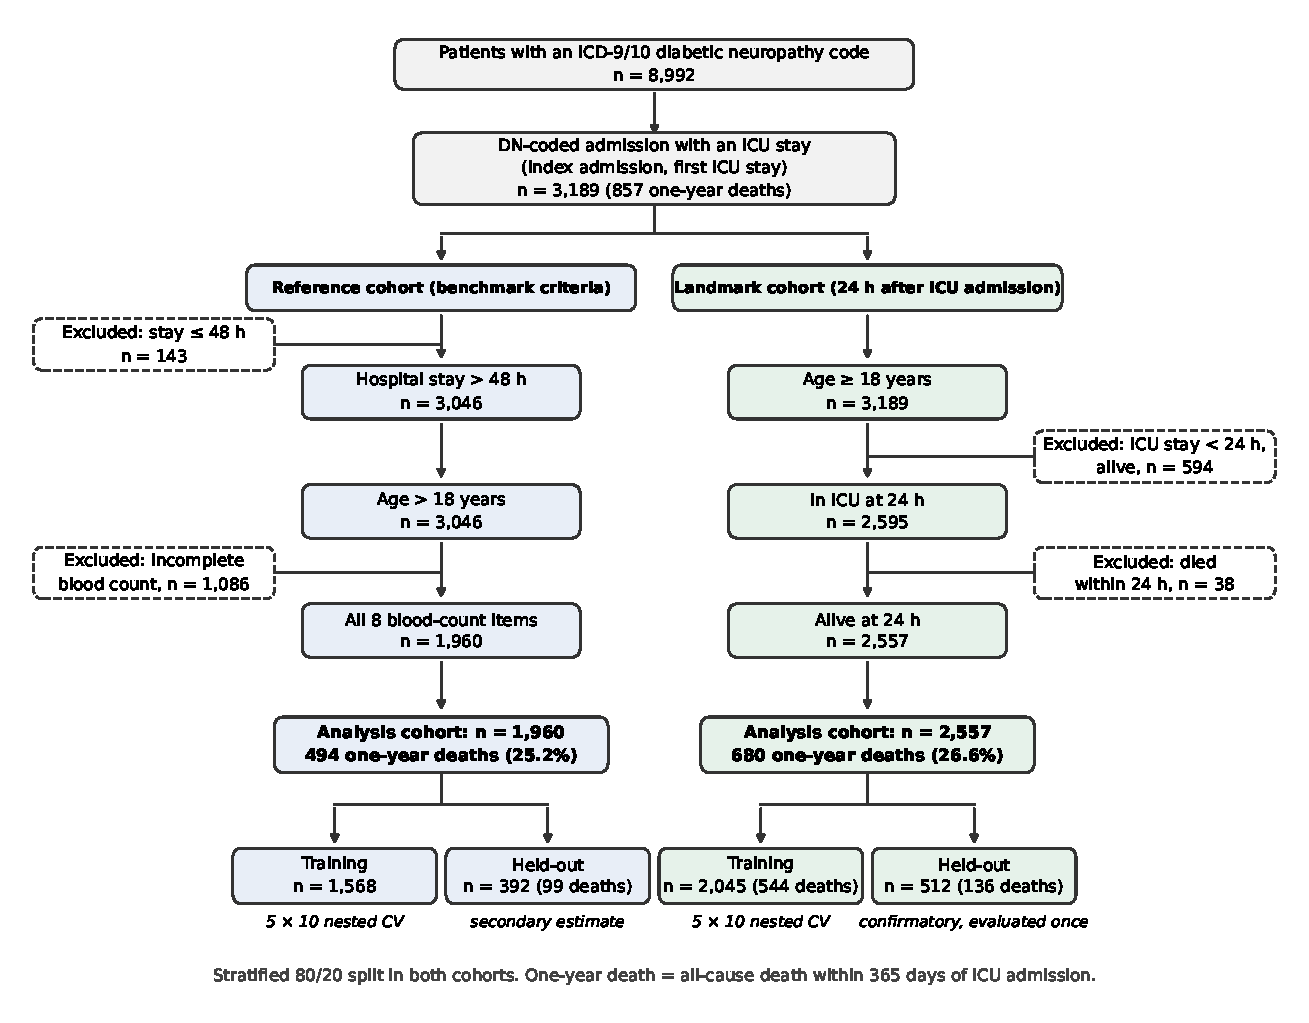
\includegraphics[width=\textwidth]{figures/fig1_cohort_flow.pdf}
\caption{Cohort flow. Both cohorts start from the same index admissions. The reference cohort applies the benchmark's inclusion criteria; the landmark cohort includes all adults alive and in the ICU 24\,h after admission.}
\label{fig:flow}
\end{figure}

\hypertarget{outcome-and-predictors-i2-i3-i4}{%
\subsection{Outcome and predictors (I2, I3,
I4)}\label{outcome-and-predictors-i2-i3-i4}}

\textbf{Outcome (I4).} The outcome was all-cause death on a date between the day
of ICU admission and 365 days later, using the in-hospital time of death when
available and the date of death from state records otherwise, compared at date
granularity. MIMIC-IV records out-of-hospital deaths up to one year after a
patient's last discharge, so every death within the 365-day window is observed.
Cause of death is not available.

\textbf{Candidate predictors.} We extracted the benchmark's 55 candidate
predictors: age and sex; six comorbidities (myocardial infarction, congestive
heart failure, chronic pulmonary disease, renal disease, hypertension, obesity);
31 laboratory summaries (glucose, anion gap, bicarbonate, creatinine, urea
nitrogen, haemoglobin, platelets, white and red cells, RDW, absolute
lymphocytes, neutrophils and monocytes, calcium, chloride, sodium, potassium,
PTT, PT, INR); four vital signs (heart rate, mean blood pressure, respiratory
rate, temperature); six severity scores (SAPS-II, APS-III, LODS, OASIS, GCS,
CCI); and six inflammatory ratios (NLR, PLR, LMR, PNR, PWR, SII). Laboratory
values were taken from 6 h before to 24 h after ICU admission and vital signs
from the first 24 h, so all predictors are available at the landmark. Every
laboratory item identifier was checked against the MIMIC-IV dictionaries.

\textbf{Units and definitions (I4).} White-cell differentials were taken as
absolute counts (10⁹/L) from the \texttt{mimic-code} blood-differential concept,
so that no patient's value mixes absolute counts with percentages. Hypertension
followed the Quan--Elixhauser definition including complicated hypertension
(ICD-9 401--405; ICD-10 I10--I13, I15, I16) \parencite{quan2005}. Under ICD
rules, hypertension with chronic kidney disease or heart failure is coded under
the complicated codes alone, so an uncomplicated-only definition labels these
patients as normotensive.

\textbf{Comorbidity timing (I3).} Diagnosis codes in MIMIC-IV carry no
timestamps, so codes of the index admission may describe acute events of the
current stay. In the landmark cohort, comorbidities were derived from all codes
of prior admissions plus the index-admission codes that remained after removing
acute-event codes (for example acute myocardial infarction, acute heart failure,
acute stroke or transient ischaemic attack, aortic dissection, acute peptic
ulcer and shock liver). The CCI was computed without its age component, because
age enters the model separately, and the chronic-disease item of SAPS-II was
recomputed over prior and index admissions.

\textbf{White-cell differential (I2).} Instead of excluding patients without a
differential, we added one binary candidate predictor,
\texttt{wbc\_diff\_missing}, equal to 1 when all three absolute cell counts were
missing. The eight differential-derived variables (three cell counts and NLR,
PLR, LMR, PNR, SII) were imputed within folds like every other variable. The
landmark analysis therefore had 56 candidate predictors.

\hypertarget{models-i6}{%
\subsection{Models (I6)}\label{models-i6}}

\textbf{Preprocessing.} Within each training set, variables with more than 20\%
missing values were dropped (the eight differential-derived variables were
exempt in the landmark cohort). Missing values were then imputed with the
training mean for continuous variables and the training mode for binary
variables and ordinal scores, and each variable was standardised to zero mean
and unit variance using training statistics. LASSO, LR and SVM used standardised
values; RF and XGBoost used imputed values on the original scale.

\textbf{Logistic regression (final model).} For patient \(i\) with predictor
vector \(\mathbf{x}_i\), the model is

\[p_i = \sigma(\beta_0 + \mathbf{x}_i^\top \boldsymbol\beta), \qquad \sigma(z) = \frac{1}{1 + e^{-z}}.\]

\emph{LASSO selection.} Variables were selected by L1-penalised LR
\parencite{tibshirani1996}, which solves

\[\min_{\beta_0, \boldsymbol\beta} \; -\frac{1}{n}\sum_{i=1}^{n}\big[y_i \log p_i + (1 - y_i)\log(1 - p_i)\big] + \lambda \lVert\boldsymbol\beta\rVert_1,\]

with the intercept unpenalised. We used scikit-learn's \texttt{liblinear}
solver, which minimises \(\lVert\boldsymbol\beta\rVert_1 + C\sum_i \ell_i\),
where \(\ell_i\) is the log-loss of patient \(i\). Dividing by \(nC\) shows that
the two problems are identical when \(C = 1/(n\lambda)\), and this conversion
was used for every \(\lambda\) (implementation details in Supplementary S9).

The solver (newGLMNET) is a coordinate-descent method of the glmnet type
\parencite{friedman2010,yuan2012}. At each outer iteration it replaces the
log-likelihood by a weighted least-squares approximation around the current
estimate, with working responses \(z_i\) and weights
\(w_i = \tilde p_i(1 - \tilde p_i)\), and then updates one coefficient at a
time. The update for coefficient \(j\) is

\[\beta_j \leftarrow \frac{S\!\left(\frac{1}{n}\sum_i w_i x_{ij}\, r_{ij},\; \lambda\right)}{\frac{1}{n}\sum_i w_i x_{ij}^2}, \qquad S(z, \lambda) = \operatorname{sign}(z)\,(|z| - \lambda)_+,\]

where \(r_{ij}\) is the partial residual of \(z_i\) that excludes predictor
\(j\). The soft-threshold operator \(S\) returns exactly zero whenever
\(|z| \le \lambda\), that is, whenever the weighted association between
predictor \(j\) and the partial residual is too weak to offset the penalty.
Coefficients are therefore set exactly to zero rather than merely shrunk, and
the predictors with non-zero coefficients form the selected set.

\emph{Choice of λ.} Over a glmnet-style grid of \(\lambda\) values
(Supplementary S9), stratified 10-fold cross-validation gave the mean held-out
binomial deviance \(\mathrm{CV}(\lambda)\) and its standard error
\(\mathrm{SE}(\lambda)\), the standard deviation across folds divided by
\(\sqrt{10}\). With \(\lambda_{\min} = \arg\min_\lambda \mathrm{CV}(\lambda)\),
the \textbf{λ.1se rule} takes the largest \(\lambda\) with
\(\mathrm{CV}(\lambda) \le \mathrm{CV}(\lambda_{\min}) + \mathrm{SE}(\lambda_{\min})\),
the sparsest model whose deviance is within one standard error of the minimum.
The predictors with non-zero coefficients at λ.1se, refitted on the whole
training data, were retained.

\emph{L2-penalised and unpenalised LR.} On the selected predictors, the
L2-penalised LR solves

\[\min_{\beta_0, \boldsymbol\beta} \; \frac{1}{n}\sum_{i=1}^{n} \ell_i + \frac{\lambda_2}{2}\lVert\boldsymbol\beta\rVert_2^2 .\]

scikit-learn minimises
\(\tfrac{1}{2}\lVert\boldsymbol\beta\rVert_2^2 + C\sum_i \ell_i\) (L-BFGS
solver, intercept unpenalised), which is the same problem with
\(\lambda_2 = 1/(nC)\). \(C\) was tuned over
\(\{0.001, 0.01, 0.1, 1, 10, 100, \infty\}\), where \(C = \infty\) removes the
penalty. The \textbf{unpenalised LR}, which corresponds to the benchmark's LR
fitted with R \texttt{glm}, was also fitted as a separate configuration.

\textbf{Random forest.} An RF averages \(B\) classification trees, each grown on
a bootstrap sample with a random subset of predictors considered at each split
\parencite{breiman2001}:

\[\hat p(\mathbf{x}) = \frac{1}{B}\sum_{b=1}^{B} T_b(\mathbf{x}),\]

where \(T_b(\mathbf{x})\) is the proportion of deaths in the leaf of tree \(b\)
that contains \(\mathbf{x}\). The tuned RF used \(B = 500\) and a grid over the
number of predictors per split, the minimum leaf size and the maximum depth.

\textbf{XGBoost.} XGBoost is an additive tree model on the log-odds scale,
\(\operatorname{logit}\hat p(\mathbf{x}) = \sum_{k=1}^{K} f_k(\mathbf{x})\),
fitted by gradient boosting with shrinkage (learning rate \(\eta\)) to minimise
\(\sum_i \ell_i + \sum_k \Omega(f_k)\) with

\[\Omega(f) = \gamma T + \tfrac{1}{2}\lambda \lVert\mathbf{w}\rVert^2,\]

where \(T\) is the number of leaves and \(\mathbf{w}\) the leaf weights
\parencite{chen2016}. \(\gamma\) and \(\lambda\) were kept at \(\gamma = 0\) and
the library default \(\lambda = 1\); the number of trees, depth, learning rate,
column and row subsampling and minimum child weight were tuned.

\textbf{Support vector machine.} The SVM solves the soft-margin problem
\(\min_{\mathbf{w}, b, \boldsymbol\xi} \tfrac{1}{2}\lVert\mathbf{w}\rVert^2 + C\sum_i \xi_i\)
subject to \(\tilde y_i(\mathbf{w}^\top\phi(\mathbf{x}_i) + b) \ge 1 - \xi_i\)
and \(\xi_i \ge 0\), with \(\tilde y_i \in \{-1, +1\}\) and the radial basis
function kernel
\(K(\mathbf{x}, \mathbf{x}') = \exp(-\gamma\lVert\mathbf{x} - \mathbf{x}'\rVert^2)\)
\parencite{cortes1995}. The SVM outputs a decision value \(f(\mathbf{x})\);
probabilities were obtained by Platt scaling,
\(\hat p = 1/(1 + \exp(A f(\mathbf{x}) + B))\), with \(A\) and \(B\) fitted by
internal cross-validation (\texttt{probability=True}) \parencite{platt1999}.
During tuning, AUROC was computed from the decision values, and the selected
configuration was then refitted with Platt scaling. \(C\) and \(\gamma\) were
tuned.

\textbf{Two configurations per family.} Each family was run (a) with the
hyperparameters reported by the benchmark and (b) tuned by grid search inside
the training data (stratified 5-fold cross-validation, AUROC as the criterion).
Together with the unpenalised LR this gives nine configurations. RF was run in
two benchmark versions, one with the literal parameters and one with R
\texttt{randomForest} defaults (nine fully grown trees), because the benchmark
lists R and Python parameter names together and the two readings imply very
different trees. All grids are listed in Supplementary S9.

\hypertarget{evaluation-framework-i5}{%
\subsection{Evaluation framework (I5)}\label{evaluation-framework-i5}}

\textbf{Repeated nested cross-validation (main estimate).} Each training set was
split into 10 stratified outer folds, and the split was repeated 5 times with
different seeds, giving \(J = 50\) outer folds. Inside every outer training
fold, the 20\% missingness rule, imputation, standardisation, LASSO (inner
stratified 10-fold cross-validation, λ.1se) and hyperparameter tuning (inner
stratified 5-fold cross-validation) were run in turn; the model was then
refitted on the whole outer training fold and evaluated on the untouched outer
validation fold (Figure 2). This estimates the performance of the whole
modelling procedure, including variable selection and tuning, rather than of one
fitted model \parencite{varma2006,cawley2010}. AUROC is reported as the mean ±
SD over the 50 outer folds. In each repeat the 10 outer validation folds were
pooled into out-of-fold (OOF) predictions covering the whole training set;
AUPRC, Brier score, calibration, decision curves and thresholds were computed
from these and averaged over the 5 repeats.

\begin{figure}[tbp]
\centering
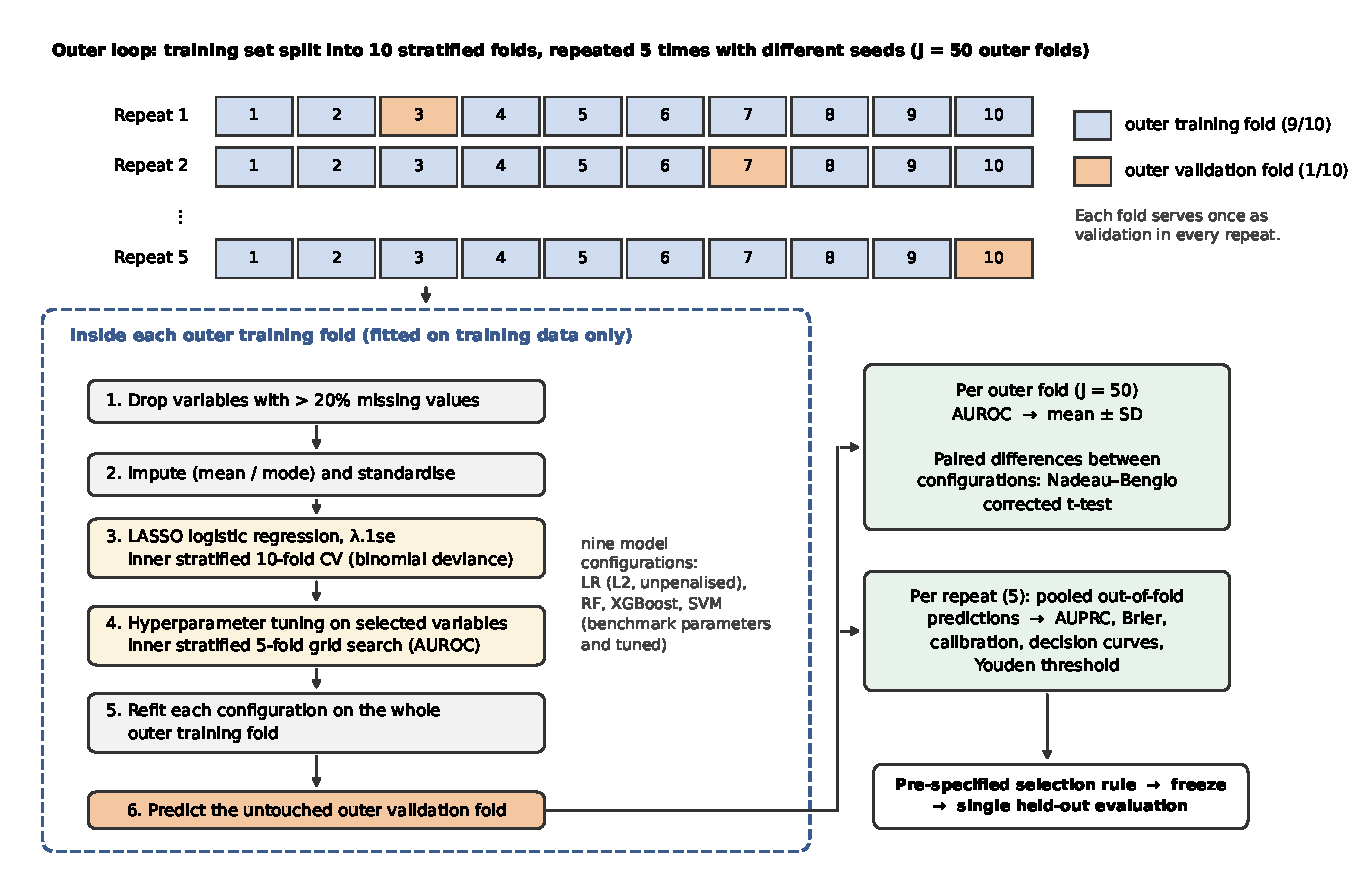
\includegraphics[width=\textwidth]{figures/fig2_nested_cv.pdf}
\caption{Repeated nested cross-validation. Every data-dependent step, including variable selection and tuning, is fitted inside each outer training fold and evaluated on the untouched outer validation fold.}
\label{fig:nestedcv}
\end{figure}

\textbf{Model comparison.} Two models evaluated on the same folds were compared
with the Nadeau--Bengio corrected resampled t-test \parencite{nadeau2003}. With
\(d_j\) the AUROC difference in outer fold \(j\), \(\bar d\) its mean and
\(\hat\sigma_d^2\) the sample variance of the \(J\) differences,

\[t = \frac{\bar d}{\sqrt{\left(\dfrac{1}{J} + \dfrac{n_{\text{test}}}{n_{\text{train}}}\right)\hat\sigma_d^2}},\]

referred to a \(t\) distribution with \(J - 1 = 49\) degrees of freedom, where
\(n_{\text{test}}/n_{\text{train}}\) is the ratio of validation-fold to
training-fold size. The term \(n_{\text{test}}/n_{\text{train}}\) inflates the
variance to account for the overlap between training sets, which the naive
paired t-test (variance \(\hat\sigma_d^2/J\)) ignores. The 95\% confidence
interval for the difference is \(\bar d \pm t_{0.975,\,J-1}\) times the
corrected standard error. In a simulation with 200 null datasets and the same
10-fold, 5-repeat design, the corrected test rejected the null hypothesis in
4.0\% of datasets and the uncorrected paired t-test in 38.0\%.

\textbf{Pre-specified model-selection rule.} (1) The configuration with the
highest mean outer AUROC is the reference M*. (2) A configuration is equivalent
to M* if its AUROC difference is at most 0.01, or at most 0.02 with a 95\%
confidence interval that includes zero. (3) If the equivalent set contains an
LR, an LR is chosen, for parsimony and interpretability. (4) If both LRs are
equivalent, the one whose pooled-OOF calibration slope is closer to 1 is chosen,
measured by the mean over repeats of \textbar ln slope\textbar{} (the
unpenalised LR on a tie). (5) The held-out set plays no part. The rule was
written before any landmark analysis was run; for the reference cohort it was
written after exploratory analyses and is therefore not blind.

\textbf{Freezing and the held-out evaluation.} After selection, the final
landmark model was fitted on the whole training set with the same pipeline
(LASSO with inner 10-fold cross-validation, then \(C\) chosen by inner 5-fold
cross-validation). Its specification, the classification threshold and
identifiers of the training data and code were recorded under version control
before the held-out set was read. The held-out evaluation was run exactly once
and was not repeated or followed by changes to the model. A tuned RF, frozen in
the same way, served as a comparator. In the reference cohort the held-out set
had been used in earlier exploratory model comparisons, so its results are
reported only as a secondary estimate.

\textbf{Held-out uncertainty.} On held-out sets, the AUROC 95\% confidence
interval used the DeLong variance \parencite{delong1988}, computed with the fast
algorithm of \textcite{sun2014}, and the two frozen models were compared with
the paired DeLong test. AUPRC confidence intervals came from a stratified
bootstrap with 2,000 resamples (percentile method).

\hypertarget{metrics-i7}{%
\subsection{Metrics (I7)}\label{metrics-i7}}

Death was the positive class throughout.

\textbf{Discrimination.} AUROC, and AUPRC computed as average precision. The
AUPRC of an uninformative model equals the prevalence \(\bar y\), which is
reported as its baseline.

\textbf{Overall accuracy.} The Brier score and the scaled Brier score
\parencite{steyerberg2010},

\[\text{Brier} = \frac{1}{n}\sum_{i=1}^{n} (\hat p_i - y_i)^2, \qquad \text{scaled Brier} = 1 - \frac{\text{Brier}}{\bar y(1 - \bar y)},\]

where \(\bar y(1 - \bar y)\) is the Brier score of a model that predicts the
prevalence for everyone, computed on the same data.

\textbf{Calibration} \parencite{vancalster2019}. A logistic recalibration model

\[\operatorname{logit} P(y = 1) = a + b \operatorname{logit}\hat p\]

was fitted to the predictions. The calibration slope is \(b\) from fitting \(a\)
and \(b\) together; the calibration intercept (calibration-in-the-large) is
\(a\) from refitting with \(b\) fixed at 1, that is, with
\(\operatorname{logit}\hat p\) as an offset. A well-calibrated model has
\(a = 0\) and \(b = 1\); \(b < 1\) means predictions that are too extreme and
\(b > 1\) predictions that are too close to the mean.

\textbf{Clinical utility.} Decision-curve analysis \parencite{vickers2006}
compares the net benefit of acting on the model at threshold probability
\(p_t\),

\[\text{NB}(p_t) = \frac{TP}{n} - \frac{FP}{n}\cdot\frac{p_t}{1 - p_t},\]

with treating everyone,
\(\text{NB}_{\text{all}}(p_t) = \bar y - (1 - \bar y)\,\frac{p_t}{1 - p_t}\),
and treating no one (\(\text{NB} = 0\)). We evaluated the 56 thresholds from
0.05 to 0.60 in steps of 0.01 and counted the thresholds at which the model's
net benefit exceeded both alternatives.

\textbf{Classification.} The threshold maximised Youden's index
\parencite{youden1950}, \(J = \text{Se} + \text{Sp} - 1\), on the pooled OOF
predictions of each repeat; the median over the 5 repeats was carried unchanged
to the held-out set. We report sensitivity, specificity, precision, F1 and the
share of patients flagged as high risk.

\hypertarget{interpretation-and-sensitivity-analyses}{%
\subsection{Interpretation and sensitivity
analyses}\label{interpretation-and-sensitivity-analyses}}

\textbf{SHAP.} For an LR on standardised predictors, the SHAP value of predictor
\(j\) (under feature independence) is

\[\phi_j(\mathbf{x}) = \beta_j\,(x_j - \mathrm{E}[x_j]),\]

on the log-odds scale, with the expectation taken over the training data used as
background \parencite{lundberg2017}. Because standardisation was fitted on the
same training data, \(\mathrm{E}[x_j] = 0\) and
\(\phi_j(\mathbf{x}) = \beta_j x_j\). Global importance is the mean \(|\phi_j|\)
over the held-out set. Tree models were explained with TreeExplainer.

\textbf{Odds ratios.} For inference, the selected predictors were refitted by
unpenalised LR on the training set. Because predictors are standardised,
\(\exp(\beta_j)\) is the odds ratio per standard deviation, with Wald 95\%
confidence interval \(\exp(\beta_j \pm 1.96\,\mathrm{SE}_j)\); for binary
predictors the coefficient was rescaled by the predictor's standard deviation to
give the odds ratio for yes versus no. Collinearity was checked with variance
inflation factors (VIF).

\textbf{Sensitivity analyses.} All were run with the full nested
cross-validation on the same outer splits as the main analysis, and compared
with it by the Nadeau--Bengio test: (i) reference cohort, comorbidities and CCI
recomputed from prior plus chronic index-admission codes (I3); (ii) reference
cohort, exclusion of patients admitted in 2020--2022, who are not covered by the
benchmark's data release (new single 80/20 split); (iii) landmark cohort,
comorbidities from prior admissions only (\emph{prior-only}, the most
conservative deployment scenario; I3); and (iv) landmark cohort, removal of all
white-cell differential variables (\emph{no-WBC-differential}; I2).

\hypertarget{exploratory-extensions}{%
\subsection{Exploratory extensions}\label{exploratory-extensions}}

The project brief proposed temporal features, comorbidity representations and a
stacking ensemble. These were evaluated after the main analysis had been
completed, on the landmark development set only (2,045 patients, 544 deaths);
the held-out set was not used. Three additions were made to the 56 static
candidates. (i) \emph{First-day trajectories}: five statistics (first-to-last
change, hourly slope, standard deviation, late-minus-early mean and number of
measurement times) for each of 25 laboratory and vital-sign series recorded
0--24 h after ICU admission, giving 125 candidates. (ii) \emph{Prior-diagnosis
burden}: four variables describing earlier admissions and their ICD codes. (iii)
\emph{Diagnosis embedding}: each patient's ICD codes from admissions that ended
before the index admission were converted to a TF-IDF document and compressed to
32 dimensions by truncated singular value decomposition, both fitted within
training folds. Stacking combined LR, RF and XGBoost base learners through an L2
LR meta-model trained on their internal 3-fold out-of-fold predictions.

To keep the computation feasible, all extension models and their static controls
used one fixed-parameter recipe (LR with \(C = 1\); RF with 200 trees of maximum
depth 10; XGBoost with 100 trees of depth 2; LASSO with 5 internal folds and 30
values of \(\lambda\)) on the same 5 × 10 outer splits as the main analysis,
with missingness screening, imputation, LASSO and the embedding refitted within
each training fold. Each extension was compared with its matched control on the
same folds by the corrected test, with Holm adjustment over 15 comparisons per
metric. Because this recipe omits inner tuning, the extensions are compared only
with their own static controls, not with Table 4.

\hypertarget{results}{%
\section{Results}\label{results}}

\hypertarget{cohort-who-the-benchmarks-criteria-exclude-i1-i2}{%
\subsection{Cohort: who the benchmark's criteria exclude (I1,
I2)}\label{cohort-who-the-benchmarks-criteria-exclude-i1-i2}}

\emph{This section shows which patients the length-of-stay and blood-count
criteria remove (I1, I2).}

Of 8,992 patients with a DN code, 3,189 had a DN-coded admission with an ICU
stay (Figure 1). The landmark cohort comprised 2,557 patients with 680 deaths
within one year (26.6\%): 594 patients whose first ICU stay ended within 24 h
and 38 who died within 24 h were excluded. The reference cohort, built with the
benchmark's criteria, comprised 1,960 patients with 494 deaths (25.2\%).

The retention at each benchmark step closely matched the benchmark (hospital
stay \textgreater{} 48 h, 95.5\% vs 95.4\%; complete blood count, 64.3\% vs
64.2\%), and the larger cohort (1,960 vs 1,313 in the benchmark) probably
reflects the extended data release (12.6\% of the reference cohort was admitted
in 2020--2022). Exclusion at the blood-count step was almost entirely due to a
missing white-cell differential (35.6\% of candidates); the core blood count was
missing in only 1\%. The landmark cohort keeps these patients: 873 (34.1\%) had
no differential, and their one-year mortality was 28.6\% (250/873), against
25.5\% (430/1,684) for patients with a differential (χ² p = 0.09). In total,
1,452 landmark patients (56.8\%) had a prior admission from which comorbidities
could be taken.

Non-survivors were older and had higher RDW, CCI and severity scores and lower
chloride (Table 2).

\begin{longtable}[]{@{}
  >{\raggedright\arraybackslash}p{(\columnwidth - 8\tabcolsep) * \real{0.2623}}
  >{\raggedright\arraybackslash}p{(\columnwidth - 8\tabcolsep) * \real{0.2049}}
  >{\raggedright\arraybackslash}p{(\columnwidth - 8\tabcolsep) * \real{0.2049}}
  >{\raggedright\arraybackslash}p{(\columnwidth - 8\tabcolsep) * \real{0.2049}}
  >{\raggedright\arraybackslash}p{(\columnwidth - 8\tabcolsep) * \real{0.1230}}@{}}
\caption{Selected baseline characteristics of the landmark cohort by one-year
outcome (median {[}IQR{]} or n {[}\%{]}; observed values before imputation).
Full tables for both cohorts are in Supplementary S3.}\tabularnewline
\toprule\noalign{}
\begin{minipage}[b]{\linewidth}\raggedright
Variable
\end{minipage} & \begin{minipage}[b]{\linewidth}\raggedright
Overall (n = 2,557)
\end{minipage} & \begin{minipage}[b]{\linewidth}\raggedright
Survivors (n = 1,877)
\end{minipage} & \begin{minipage}[b]{\linewidth}\raggedright
Non-survivors (n = 680)
\end{minipage} & \begin{minipage}[b]{\linewidth}\raggedright
p
\end{minipage} \\
\midrule\noalign{}
\endfirsthead
\toprule\noalign{}
\begin{minipage}[b]{\linewidth}\raggedright
Variable
\end{minipage} & \begin{minipage}[b]{\linewidth}\raggedright
Overall (n = 2,557)
\end{minipage} & \begin{minipage}[b]{\linewidth}\raggedright
Survivors (n = 1,877)
\end{minipage} & \begin{minipage}[b]{\linewidth}\raggedright
Non-survivors (n = 680)
\end{minipage} & \begin{minipage}[b]{\linewidth}\raggedright
p
\end{minipage} \\
\midrule\noalign{}
\endhead
\bottomrule\noalign{}
\endlastfoot
Age, years & 67 (58--75) & 65 (57--73) & 71 (63--79) & \textless0.001 \\
Male sex & 1,520 (59.44\%) & 1,097 (58.44\%) & 423 (62.21\%) & 0.087 \\
Congestive heart failure & 1,178 (46.07\%) & 775 (41.29\%) & 403 (59.26\%) &
\textless0.001 \\
Renal disease & 1,299 (50.80\%) & 877 (46.72\%) & 422 (62.06\%) &
\textless0.001 \\
Obesity (coded) & 859 (33.59\%) & 664 (35.38\%) & 195 (28.68\%) & 0.002 \\
CCI (without age) & 5 (4--7) & 5 (3--6) & 6 (5--8) & \textless0.001 \\
RDW, \% & 14.65 (13.60--16.20) & 14.30 (13.40--15.65) & 15.81 (14.49--17.63) &
\textless0.001 \\
Chloride (max), mmol/L & 105 (100--109) & 106 (101--109) & 103 (98--108) &
\textless0.001 \\
Anion gap (min), mmol/L & 13 (10--15) & 12 (10--14) & 14 (11--17) &
\textless0.001 \\
Urea nitrogen (min), mg/dL & 23 (15--39) & 21 (14--34) & 32 (20--53) &
\textless0.001 \\
Lymphocytes, 10⁹/L † & 1.27 (0.79--1.95) & 1.39 (0.87--2.08) & 0.95 (0.60--1.47)
& \textless0.001 \\
Respiratory rate, /min & 18.28 (16.43--20.62) & 18.08 (16.32--20.20) & 19.12
(16.99--21.75) & \textless0.001 \\
SAPS-II & 36 (29--45) & 34 (27--42) & 42 (35--52.25) & \textless0.001 \\
APS-III & 45 (35--57) & 42 (34--53) & 54 (43--67) & \textless0.001 \\
OASIS & 30 (25--36) & 30 (24--35) & 33.5 (27--40) & \textless0.001 \\
No white-cell differential & 873 (34.14\%) & 623 (33.19\%) & 250 (36.76\%) &
0.092 \\
Prior admission & 1,452 (56.79\%) & 1,028 (54.77\%) & 424 (62.35\%) &
\textless0.001 \\
\end{longtable}

† 34.1\% missing (no differential performed).

\hypertarget{definition-errors-in-the-benchmark-i4}{%
\subsection{Definition errors in the benchmark
(I4)}\label{definition-errors-in-the-benchmark-i4}}

\emph{This section gives the evidence for the three definition problems
addressed by I4. The comparisons use the reference cohort, which follows the
benchmark's criteria.}

\textbf{Mortality.} One-year mortality from ICU admission was 25.2\% in the
reference cohort, against 38.2\% in the benchmark. In-hospital mortality was
only 7.1\%, so the benchmark's figure cannot be in-hospital mortality, although
its abstract names in-hospital death. Counting every recorded date of death
regardless of timing gave 42.8\%, the same order as the benchmark, and 49\% of
patients with an out-of-hospital date of death died more than 365 days after ICU
admission. The benchmark may therefore have used an outcome without a fixed
follow-up window; because it does not state its definition, this cannot be
confirmed.

\textbf{White-cell differential units.} The benchmark reported lymphocytes of
3.69 (1.27--118.32), neutrophils of 23.90 (8.63--831.30) and monocytes of 2.00
(0.60--43.64) × 10⁹/L, which are physiologically implausible. With absolute
counts we obtained 1.24 (0.77--1.91), 8.59 (5.99--12.57) and 0.55 (0.35--0.84).
The pattern of the derived ratios indicates mixing of scales across patients.
Ratios that are unaffected when a patient's three cell counts share one scale
agreed with the benchmark (NLR 6.82 vs 6.80; LMR 2.31 vs 2.42; SII 1,336 vs
1,342), whereas ratios that combine platelets with a differential count did not
(PLR 159 vs 36; PNR 22 vs 6.6). When we deliberately mixed all differential
items, PLR and PNR fell to 24.00 and 3.67, moving towards the benchmark's
values. With correct units, neutrophils were selected by LASSO only at λ.min,
not at λ.1se, and were not among the five most important predictors, whereas
they ranked second in the benchmark.

\textbf{Hypertension.} Hypertension prevalence was 84.6\% under the full
Quan--Elixhauser definition, against 37.3\% in the benchmark; counting only
uncomplicated hypertension codes gave 35.4\%, close to the benchmark. The narrow
definition reverses the apparent effect. Under the full definition, hypertension
was unrelated to one-year death (unadjusted OR 1.07, 95\% CI 0.80--1.42). Under
the uncomplicated definition it appeared protective (OR 0.49, 0.39--0.62),
because the 964 patients who had only complicated codes, and were therefore
coded as normotensive, had a one-year mortality of 31.3\% (OR 1.91, 1.55--2.35).
LASSO did not select hypertension under either definition, and the selected
variables were identical, so the models were unaffected.

\hypertarget{the-benchmark-pipeline-under-leakage-free-evaluation-i5-i6}{%
\subsection{The benchmark pipeline under leakage-free evaluation (I5,
I6)}\label{the-benchmark-pipeline-under-leakage-free-evaluation-i5-i6}}

\emph{This section applies the improved evaluation (I5) and tuning (I6) to the
reference cohort, to test the benchmark's own model ranking. Full results are in
Supplementary S2.}

LASSO on the reference training set selected 12 variables at λ.1se (λ = 0.02667,
against 0.02687 in the benchmark), seven of which overlapped with the
benchmark's 12 (age, anion gap, RDW, chloride, PT, APS-III, CCI); at λ.min the
overlap was 11 of 12.

Under nested cross-validation, six configurations were equivalent to the best
model, with AUROC 0.786--0.791 (Table 3). The benchmark's two RF configurations
and its SVM were significantly worse, with confidence intervals for the
difference that excluded zero. Among the benchmark-parameter models, only
XGBoost matched the best model.

\begin{longtable}[]{@{}
  >{\raggedright\arraybackslash}p{(\columnwidth - 12\tabcolsep) * \real{0.2417}}
  >{\raggedright\arraybackslash}p{(\columnwidth - 12\tabcolsep) * \real{0.1750}}
  >{\raggedright\arraybackslash}p{(\columnwidth - 12\tabcolsep) * \real{0.1333}}
  >{\raggedright\arraybackslash}p{(\columnwidth - 12\tabcolsep) * \real{0.0917}}
  >{\raggedright\arraybackslash}p{(\columnwidth - 12\tabcolsep) * \real{0.0917}}
  >{\raggedright\arraybackslash}p{(\columnwidth - 12\tabcolsep) * \real{0.1083}}
  >{\raggedright\arraybackslash}p{(\columnwidth - 12\tabcolsep) * \real{0.1583}}@{}}
\caption{Reference cohort: nested cross-validation on the training set (1,568
patients; 5 × 10 folds) and the benchmark's reported validation
AUCs.}\tabularnewline
\toprule\noalign{}
\begin{minipage}[b]{\linewidth}\raggedright
Model
\end{minipage} & \begin{minipage}[b]{\linewidth}\raggedright
Benchmark validation AUC \parencite{huang2025}
\end{minipage} & \begin{minipage}[b]{\linewidth}\raggedright
Nested-CV AUROC (mean ± SD)
\end{minipage} & \begin{minipage}[b]{\linewidth}\raggedright
AUPRC
\end{minipage} & \begin{minipage}[b]{\linewidth}\raggedright
Brier
\end{minipage} & \begin{minipage}[b]{\linewidth}\raggedright
Calibration slope
\end{minipage} & \begin{minipage}[b]{\linewidth}\raggedright
ΔAUROC vs best (95\% CI)
\end{minipage} \\
\midrule\noalign{}
\endfirsthead
\toprule\noalign{}
\begin{minipage}[b]{\linewidth}\raggedright
Model
\end{minipage} & \begin{minipage}[b]{\linewidth}\raggedright
Benchmark validation AUC \parencite{huang2025}
\end{minipage} & \begin{minipage}[b]{\linewidth}\raggedright
Nested-CV AUROC (mean ± SD)
\end{minipage} & \begin{minipage}[b]{\linewidth}\raggedright
AUPRC
\end{minipage} & \begin{minipage}[b]{\linewidth}\raggedright
Brier
\end{minipage} & \begin{minipage}[b]{\linewidth}\raggedright
Calibration slope
\end{minipage} & \begin{minipage}[b]{\linewidth}\raggedright
ΔAUROC vs best (95\% CI)
\end{minipage} \\
\midrule\noalign{}
\endhead
\bottomrule\noalign{}
\endlastfoot
XGBoost (benchmark parameters) & 0.732 & \textbf{0.791 ± 0.035} & 0.559 & 0.150
& 0.96 & reference \\
XGBoost (tuned) & --- & 0.790 ± 0.035 & 0.558 & 0.150 & 0.96 & 0.000 (−0.005,
0.006) \\
LR (L2, tuned) & --- & 0.788 ± 0.036 & 0.536 & 0.154 & 1.19 & 0.002 (−0.009,
0.014) \\
RF (tuned) & --- & 0.788 ± 0.036 & 0.548 & 0.154 & 1.48 & 0.002 (−0.006,
0.011) \\
SVM (tuned) & --- & 0.788 ± 0.036 & 0.541 & 0.153 & 0.90 & 0.003 (−0.008,
0.014) \\
LR (unpenalised) & 0.773 & 0.786 ± 0.035 & 0.550 & 0.151 & 0.85 & 0.005 (−0.007,
0.016) \\
RF (benchmark, literal parameters) & 0.780 & 0.767 ± 0.038 & 0.519 & 0.156 &
0.94 & 0.024 (0.006, 0.041) \\
RF (benchmark, R defaults) & 0.780 & 0.724 ± 0.039 & 0.440 & 0.171 & 0.15 &
0.066 (0.043, 0.090) \\
SVM (benchmark parameters) & 0.679 & 0.723 ± 0.044 & 0.497 & 0.163 & 0.96 &
0.068 (0.042, 0.093) \\
\end{longtable}

AUPRC baseline = 0.252. The first six rows are equivalent to the reference under
the pre-specified rule, which selected the unpenalised LR (for this cohort the
rule was not blind; Section 2.5). On the secondary held-out set (392 patients),
the unpenalised LR had AUROC 0.803 (0.753--0.853) and calibration slope 0.96.

Three further results bear on the benchmark's pipeline.

\begin{itemize}
\tightlist
\item
  \textbf{RF overfitting (I6).} With R defaults (nine fully grown trees), the RF
  reproduced the benchmark's training AUC of 0.999 but had a validation AUC of
  0.756 on a single split, a nested-CV AUROC of 0.724 and a calibration slope of
  0.15, indicating severely overconfident predictions. With the literal
  parameters the training AUC was only 0.887. The benchmark's 0.999 is therefore
  consistent with fully grown trees, although other causes cannot be ruled out.
\item
  \textbf{Variable selection outside cross-validation (I5).} Treating the LASSO
  selection as fixed, as the benchmark did, overstated the cross-validated AUROC
  of the unpenalised LR by 0.011 (0.793 vs 0.781), and of the nine
  configurations by 0.008--0.030 (single repeat of 10-fold cross-validation).
\item
  \textbf{Preprocessing leakage (I5).} Fitting imputation and standardisation on
  all data, as in the benchmark, did not change the LASSO selection and changed
  model metrics by at most 0.001. Missingness was at most 7.04\%, which probably
  explains why this form of leakage had negligible impact here.
\end{itemize}

A single validation set could not rank the models: on the 392-patient validation
set, no pair of tuned models differed significantly after Holm correction
(smallest adjusted p = 0.13).

\hypertarget{improved-landmark-model-main-result}{%
\subsection{Improved landmark model (main
result)}\label{improved-landmark-model-main-result}}

\emph{This section reports the main estimate of the improved framework (I1--I6
combined) for the landmark cohort.}

\textbf{Nested cross-validation.} LASSO selected 13--23 of the 56 candidates per
outer fold (median 17). Age, anion gap, CCI, OASIS, APS-III, respiratory rate,
RDW, maximum chloride and obesity were selected in all 50 folds;
\texttt{wbc\_diff\_missing} was selected in 13 of 50. Of the six comorbidities,
only obesity was ever selected. Six configurations were again equivalent (AUROC
0.794--0.801; Table 4), and the benchmark's RF and SVM configurations were again
not.

\begin{longtable}[]{@{}
  >{\raggedright\arraybackslash}p{(\columnwidth - 10\tabcolsep) * \real{0.2893}}
  >{\raggedright\arraybackslash}p{(\columnwidth - 10\tabcolsep) * \real{0.1653}}
  >{\raggedright\arraybackslash}p{(\columnwidth - 10\tabcolsep) * \real{0.1074}}
  >{\raggedright\arraybackslash}p{(\columnwidth - 10\tabcolsep) * \real{0.1074}}
  >{\raggedright\arraybackslash}p{(\columnwidth - 10\tabcolsep) * \real{0.1322}}
  >{\raggedright\arraybackslash}p{(\columnwidth - 10\tabcolsep) * \real{0.1983}}@{}}
\caption{Landmark cohort: nested cross-validation on the training set (2,045
patients; 5 × 10 folds).}\tabularnewline
\toprule\noalign{}
\begin{minipage}[b]{\linewidth}\raggedright
Model
\end{minipage} & \begin{minipage}[b]{\linewidth}\raggedright
AUROC (mean ± SD)
\end{minipage} & \begin{minipage}[b]{\linewidth}\raggedright
AUPRC
\end{minipage} & \begin{minipage}[b]{\linewidth}\raggedright
Brier
\end{minipage} & \begin{minipage}[b]{\linewidth}\raggedright
Calibration slope
\end{minipage} & \begin{minipage}[b]{\linewidth}\raggedright
ΔAUROC vs best (95\% CI)
\end{minipage} \\
\midrule\noalign{}
\endfirsthead
\toprule\noalign{}
\begin{minipage}[b]{\linewidth}\raggedright
Model
\end{minipage} & \begin{minipage}[b]{\linewidth}\raggedright
AUROC (mean ± SD)
\end{minipage} & \begin{minipage}[b]{\linewidth}\raggedright
AUPRC
\end{minipage} & \begin{minipage}[b]{\linewidth}\raggedright
Brier
\end{minipage} & \begin{minipage}[b]{\linewidth}\raggedright
Calibration slope
\end{minipage} & \begin{minipage}[b]{\linewidth}\raggedright
ΔAUROC vs best (95\% CI)
\end{minipage} \\
\midrule\noalign{}
\endhead
\bottomrule\noalign{}
\endlastfoot
LR (L2, tuned) & \textbf{0.801 ± 0.026} & 0.594 & 0.151 & 1.11 & reference \\
LR (unpenalised) & 0.799 ± 0.026 & 0.592 & 0.151 & 0.90 & 0.003 (−0.001,
0.006) \\
SVM (tuned) & 0.798 ± 0.028 & 0.584 & 0.153 & 0.92 & 0.004 (−0.002, 0.009) \\
RF (tuned) & 0.797 ± 0.028 & 0.591 & 0.155 & 1.46 & 0.004 (−0.005, 0.014) \\
XGBoost (tuned) & 0.795 ± 0.028 & 0.596 & 0.152 & 0.99 & 0.006 (−0.004,
0.015) \\
XGBoost (benchmark parameters) & 0.794 ± 0.029 & 0.597 & 0.152 & 1.02 & 0.008
(−0.002, 0.017) \\
RF (benchmark, literal parameters) & 0.781 ± 0.029 & 0.560 & 0.157 & 1.09 &
0.020 (0.008, 0.033) \\
SVM (benchmark parameters) & 0.756 ± 0.035 & 0.550 & 0.161 & 0.98 & 0.046
(0.027, 0.065) \\
RF (benchmark, R defaults) & 0.740 ± 0.037 & 0.488 & 0.170 & 0.18 & 0.061
(0.039, 0.083) \\
\end{longtable}

AUPRC baseline = 0.266.

\textbf{Model selection.} The L2-penalised LR had the highest mean AUROC and was
the reference M*. Both LRs were in the equivalent set, and the rule chose the L2
LR on calibration (mean \textbar ln slope\textbar{} 0.102 vs 0.109). This was a
near tie: the two LRs differed in AUROC by 0.003, their slopes deviated from 1
by similar amounts in opposite directions (1.11 and 0.90), and the unpenalised
LR was closer to 1 in three of five repeats. No claim of better discrimination
is made for the selected model. Inner tuning chose C = 0.01 in all 50 folds.

\textbf{Final model.} Refitted on the whole training set (544 events), LASSO
selected 22 variables (λ.1se = 0.0168; 24.7 events per selected variable) and
inner tuning chose C = 0.01. The frozen model and the tuned RF comparator were
evaluated once on the held-out set (512 patients, 136 deaths; Table 5, Figure
3).

\begin{longtable}[]{@{}
  >{\raggedright\arraybackslash}p{(\columnwidth - 4\tabcolsep) * \real{0.4167}}
  >{\raggedright\arraybackslash}p{(\columnwidth - 4\tabcolsep) * \real{0.2917}}
  >{\raggedright\arraybackslash}p{(\columnwidth - 4\tabcolsep) * \real{0.2917}}@{}}
\caption{Landmark cohort: confirmatory held-out evaluation of the frozen
models.}\tabularnewline
\toprule\noalign{}
\begin{minipage}[b]{\linewidth}\raggedright
Metric
\end{minipage} & \begin{minipage}[b]{\linewidth}\raggedright
LR (L2), selected
\end{minipage} & \begin{minipage}[b]{\linewidth}\raggedright
RF (tuned), comparator
\end{minipage} \\
\midrule\noalign{}
\endfirsthead
\toprule\noalign{}
\begin{minipage}[b]{\linewidth}\raggedright
Metric
\end{minipage} & \begin{minipage}[b]{\linewidth}\raggedright
LR (L2), selected
\end{minipage} & \begin{minipage}[b]{\linewidth}\raggedright
RF (tuned), comparator
\end{minipage} \\
\midrule\noalign{}
\endhead
\bottomrule\noalign{}
\endlastfoot
AUROC (95\% CI) & 0.750 (0.702--0.797) & 0.752 (0.704--0.799) \\
AUPRC (95\% CI; baseline 0.266) & 0.533 (0.459--0.611) & 0.529 (0.460--0.615) \\
Brier / scaled Brier & 0.165 / 0.153 & 0.164 / 0.161 \\
Calibration intercept / slope & +0.049 / 0.82 & +0.013 / 1.14 \\
Threshold (OOF Youden) & 0.258 & 0.241 \\
Sensitivity / specificity & 0.684 / 0.697 & 0.779 / 0.596 \\
Precision / F1 & 0.449 / 0.542 & 0.411 / 0.538 \\
Flagged as high risk & 40.4\% & 50.4\% \\
\end{longtable}

Paired DeLong test, LR − RF: −0.002 (−0.021, 0.016), p = 0.83.

\begin{figure}[tbp]
\centering
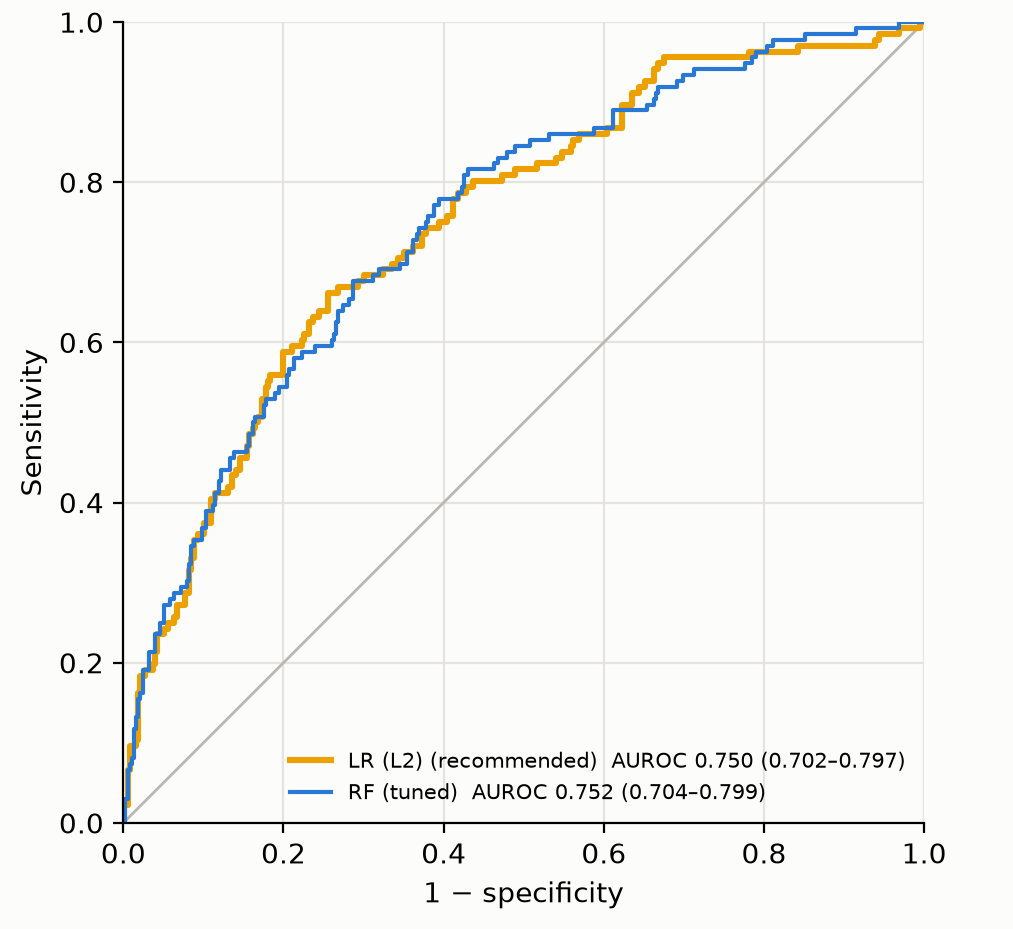
\includegraphics[height=5.2cm]{figures/figC1_roc_clin_holdout.png}\hfill
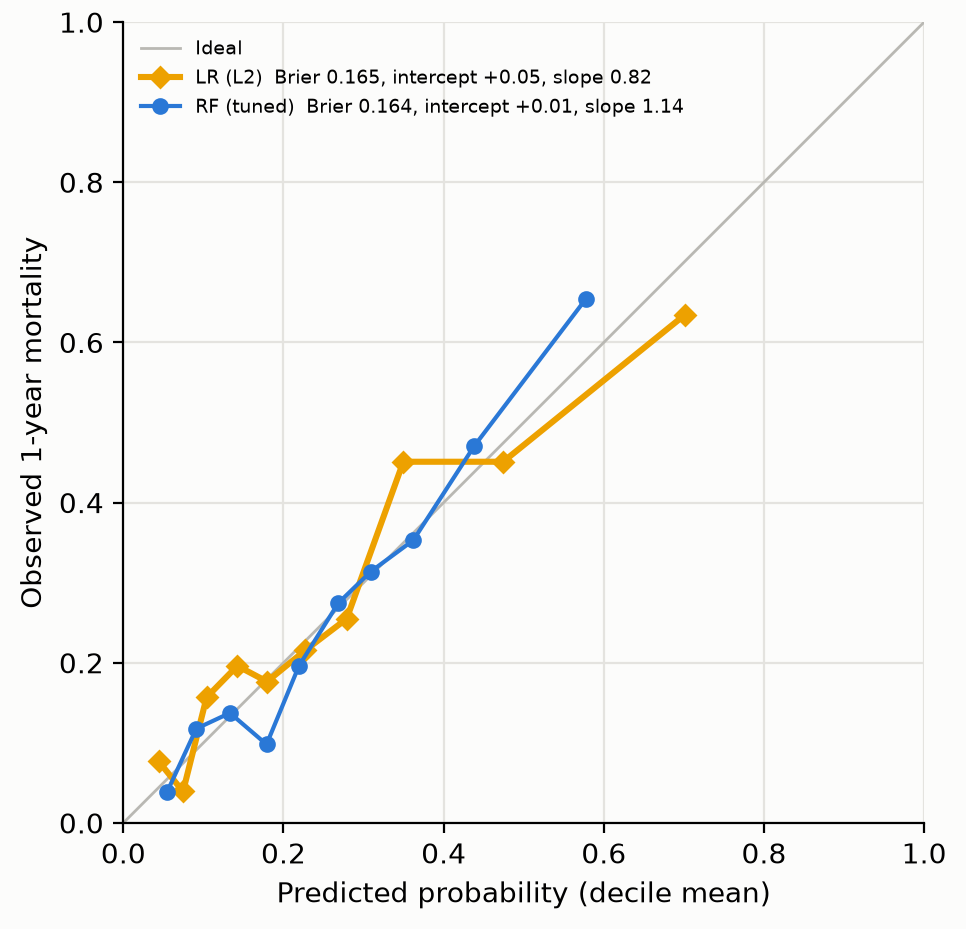
\includegraphics[height=5.2cm]{figures/figC2_calibration_clin_holdout.png}\\[4pt]
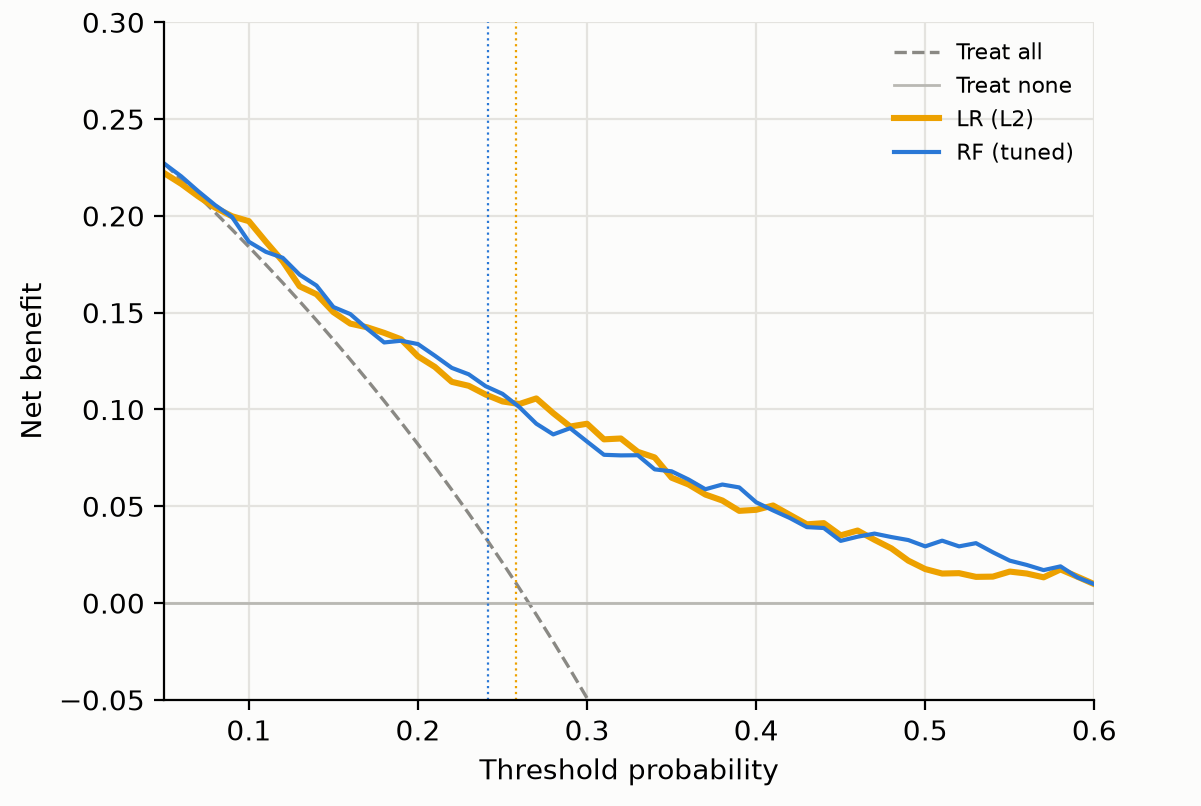
\includegraphics[height=5.6cm]{figures/figC3_dca_clin_holdout.png}
\caption{Frozen landmark models on the held-out set (512 patients, 136 deaths): (a) ROC curves, (b) calibration, (c) decision curves, with dotted vertical lines marking each model's frozen Youden threshold.}
\label{fig:holdout}
\end{figure}

\textbf{Held-out estimate below the cross-validated estimate.} The held-out
AUROC was about 0.05 below the nested-CV estimate, and the nested-CV estimate
lay above the upper limit of the held-out confidence interval. The RF comparator
dropped in parallel (0.797 to 0.752). Post-hoc checks, which changed neither the
frozen model nor the confirmatory result, did not point to overfitting: the
frozen LR's apparent training AUROC was 0.817, only 0.016 above nested CV. When
the OOF predictions were resampled 10,000 times to the held-out composition (136
deaths, 376 survivors), the mean AUROC was 0.800 (SD 0.021; 2.5th percentile
0.755), and 1.4\% of resamples were at or below 0.750; this simulation ignores
refitting variability and so understates the total variation. The largest
standardised mean difference between training and held-out sets across the 22
selected variables was 0.11. The gap is therefore more likely sampling variation
in a 512-patient set than overfitting, although other causes cannot be excluded.
As pre-specified, the model was not changed and the evaluation was not repeated;
taken together, the landmark model's discrimination lies between 0.75 and 0.80.

\hypertarget{calibration-and-clinical-utility-i7}{%
\subsection{Calibration and clinical utility
(I7)}\label{calibration-and-clinical-utility-i7}}

\emph{This section reports the metrics added under I7.}

\textbf{Calibration.} Out of fold, the selected L2 LR had a calibration slope of
1.11 (predictions slightly too close to the mean) and the unpenalised LR 0.90.
On the held-out set, the L2 LR's slope was 0.82 with intercept +0.049, so its
predictions were slightly too extreme, the opposite direction to the
cross-validated estimate. The tuned RF had out-of-fold slopes of 1.46 in the
landmark cohort and 1.48 in the reference cohort (predictions shrunk towards the
mean), and 1.14 on the held-out set. The benchmark's R-default RF had slopes of
0.18 and 0.15. Discrimination alone would not have revealed these differences,
and the instability of the selected model's slope means that it must be
recalibrated before use in a new population.

\textbf{Overall accuracy.} The held-out Brier score of the L2 LR was 0.165
(scaled Brier 0.153), similar to the RF comparator (0.164; 0.161).

\textbf{Decision curves.} On the held-out set, the L2 LR had net benefit above
both treat-all and treat-none at 53 of 56 thresholds (0.08--0.60), and the tuned
RF at 55 of 56 (0.06--0.60). In the reference cohort, the unpenalised LR was
above both at 56 of 56 thresholds in nested cross-validation and on its held-out
set.

\textbf{Classification.} At its out-of-fold Youden threshold (0.258), the
landmark LR flagged 40.4\% of held-out patients as high risk, of whom 44.9\%
died within one year (precision 0.449), with sensitivity 0.684 and specificity
0.697. A threshold of 0.5 would be inappropriate at this prevalence: in the
reference cohort it flagged only 16.3\% of patients, with sensitivity 0.44. The
benchmark reported precision 0.735 and recall 0.858 for its RF; these values are
internally consistent only if survival was the positive class, so they are not
comparable with ours.

\hypertarget{what-each-improvement-changed-sensitivity-analyses}{%
\subsection{What each improvement changed (sensitivity
analyses)}\label{what-each-improvement-changed-sensitivity-analyses}}

\emph{This section isolates the effect of the comorbidity-timing (I3) and
white-cell differential (I2) modifications, and of the data release.}

\begin{longtable}[]{@{}
  >{\raggedright\arraybackslash}p{(\columnwidth - 8\tabcolsep) * \real{0.1250}}
  >{\raggedright\arraybackslash}p{(\columnwidth - 8\tabcolsep) * \real{0.3250}}
  >{\raggedright\arraybackslash}p{(\columnwidth - 8\tabcolsep) * \real{0.1750}}
  >{\raggedright\arraybackslash}p{(\columnwidth - 8\tabcolsep) * \real{0.1250}}
  >{\raggedright\arraybackslash}p{(\columnwidth - 8\tabcolsep) * \real{0.2500}}@{}}
\caption{Sensitivity analyses (nested cross-validation on the same outer splits;
ΔAUROC = sensitivity − main, Nadeau--Bengio 95\% CI).}\tabularnewline
\toprule\noalign{}
\begin{minipage}[b]{\linewidth}\raggedright
Cohort
\end{minipage} & \begin{minipage}[b]{\linewidth}\raggedright
Analysis
\end{minipage} & \begin{minipage}[b]{\linewidth}\raggedright
Model
\end{minipage} & \begin{minipage}[b]{\linewidth}\raggedright
AUROC
\end{minipage} & \begin{minipage}[b]{\linewidth}\raggedright
ΔAUROC (95\% CI)
\end{minipage} \\
\midrule\noalign{}
\endfirsthead
\toprule\noalign{}
\begin{minipage}[b]{\linewidth}\raggedright
Cohort
\end{minipage} & \begin{minipage}[b]{\linewidth}\raggedright
Analysis
\end{minipage} & \begin{minipage}[b]{\linewidth}\raggedright
Model
\end{minipage} & \begin{minipage}[b]{\linewidth}\raggedright
AUROC
\end{minipage} & \begin{minipage}[b]{\linewidth}\raggedright
ΔAUROC (95\% CI)
\end{minipage} \\
\midrule\noalign{}
\endhead
\bottomrule\noalign{}
\endlastfoot
Reference & Comorbidity timing & LR (unpenalised) & 0.787 & +0.001 (−0.006,
0.008) \\
Reference & Comorbidity timing & RF (tuned) & 0.790 & +0.002 (−0.006, 0.010) \\
Landmark & Prior-admission comorbidities only & LR (L2) & 0.787 & −0.014
(−0.023, −0.005) \\
Landmark & Prior-admission comorbidities only & RF (tuned) & 0.789 & −0.008
(−0.016, −0.0001) \\
Landmark & No white-cell differential & LR (L2) & 0.802 & +0.001 (−0.005,
0.007) \\
Landmark & No white-cell differential & RF (tuned) & 0.795 & −0.002 (−0.010,
0.005) \\
\end{longtable}

\textbf{Comorbidity timing (I3).} In the reference cohort, recomputing
comorbidities from prior plus chronic index-admission codes changed the CCI for
843 patients, and 304 of 611 myocardial-infarction diagnoses (about half) came
only from acute index-admission codes. Discrimination was nevertheless
unchanged, and CCI was still selected in every fold. In the landmark cohort,
using prior admissions only lowered AUROC by 0.014 for the LR, with a confidence
interval excluding zero. The largest change was in obesity, whose selection fell
from 50 to 4 of 50 folds. This prior-only estimate (about 0.787) is the most
conservative deployment scenario, because it does not assume that chronic
index-admission codes were present at admission.

\textbf{White-cell differential (I2).} Removing all eight differential
variables, including the missingness indicator, did not change discrimination,
AUPRC, Brier score or calibration, and reduced the median number of selected
variables from 17 to 13. The benefit of I2 is therefore in the cohort it allows,
not in discrimination.

\textbf{Data release.} Excluding the 247 patients admitted in 2020--2022 from
the reference cohort (new single 80/20 split) gave validation AUROCs of 0.799
for the unpenalised LR and 0.802 for the tuned RF, against 0.803 and 0.793 in
the main split, and RDW and CCI remained the two most important predictors of
the LR.

\hypertarget{predictors-and-interpretation}{%
\subsection{Predictors and interpretation}\label{predictors-and-interpretation}}

\emph{This section compares the predictors identified by the benchmark and by
our models.}

RDW and CCI ranked first and second in every model, and age ranked third in both
LRs; the tuned RF ranked SAPS-II third (Table 7; Figure 4). In the landmark
model (unpenalised refit, odds ratio per SD), higher risk was associated with
RDW (OR 1.67, 95\% CI 1.47--1.89), age (1.50, 1.30--1.75), CCI (1.44,
1.27--1.63), APS-III (1.38, 1.14--1.67), OASIS (1.23, 1.04--1.46), respiratory
rate (1.20, 1.06--1.34) and minimum calcium (1.16, 1.02--1.32). Lower risk was
associated with higher maximum chloride (0.82, 0.73--0.94) and coded obesity
(yes vs no, 0.63, 0.49--0.81). Male sex (1.31, 1.03--1.66) and a missing
white-cell differential (1.33, 1.04--1.71) were associated with higher risk. All
variance inflation factors were below 5 (largest 4.74, SAPS-II), and SAPS-II,
LODS, NLR and SII were not significant once the other scores and ratios were
included.

\begin{longtable}[]{@{}
  >{\raggedright\arraybackslash}p{(\columnwidth - 8\tabcolsep) * \real{0.1500}}
  >{\raggedright\arraybackslash}p{(\columnwidth - 8\tabcolsep) * \real{0.2917}}
  >{\raggedright\arraybackslash}p{(\columnwidth - 8\tabcolsep) * \real{0.2083}}
  >{\raggedright\arraybackslash}p{(\columnwidth - 8\tabcolsep) * \real{0.1917}}
  >{\raggedright\arraybackslash}p{(\columnwidth - 8\tabcolsep) * \real{0.1583}}@{}}
\caption{Top-5 predictors by mean \textbar SHAP\textbar.}\tabularnewline
\toprule\noalign{}
\begin{minipage}[b]{\linewidth}\raggedright
Rank
\end{minipage} & \begin{minipage}[b]{\linewidth}\raggedright
Benchmark (RF) \parencite{huang2025}
\end{minipage} & \begin{minipage}[b]{\linewidth}\raggedright
Reference: LR (unpenalised)
\end{minipage} & \begin{minipage}[b]{\linewidth}\raggedright
Reference: RF (tuned)
\end{minipage} & \begin{minipage}[b]{\linewidth}\raggedright
Landmark: LR (L2)
\end{minipage} \\
\midrule\noalign{}
\endfirsthead
\toprule\noalign{}
\begin{minipage}[b]{\linewidth}\raggedright
Rank
\end{minipage} & \begin{minipage}[b]{\linewidth}\raggedright
Benchmark (RF) \parencite{huang2025}
\end{minipage} & \begin{minipage}[b]{\linewidth}\raggedright
Reference: LR (unpenalised)
\end{minipage} & \begin{minipage}[b]{\linewidth}\raggedright
Reference: RF (tuned)
\end{minipage} & \begin{minipage}[b]{\linewidth}\raggedright
Landmark: LR (L2)
\end{minipage} \\
\midrule\noalign{}
\endhead
\bottomrule\noalign{}
\endlastfoot
1 & RDW & RDW & RDW & RDW \\
2 & Neutrophils & CCI & CCI & CCI \\
3 & CCI & Age & SAPS-II & Age \\
4 & Chloride (max) & APS-III & APS-III & APS-III \\
5 & PT (min) & OASIS & Chloride (max) & Obesity \\
\end{longtable}

\begin{figure}[tbp]
\centering
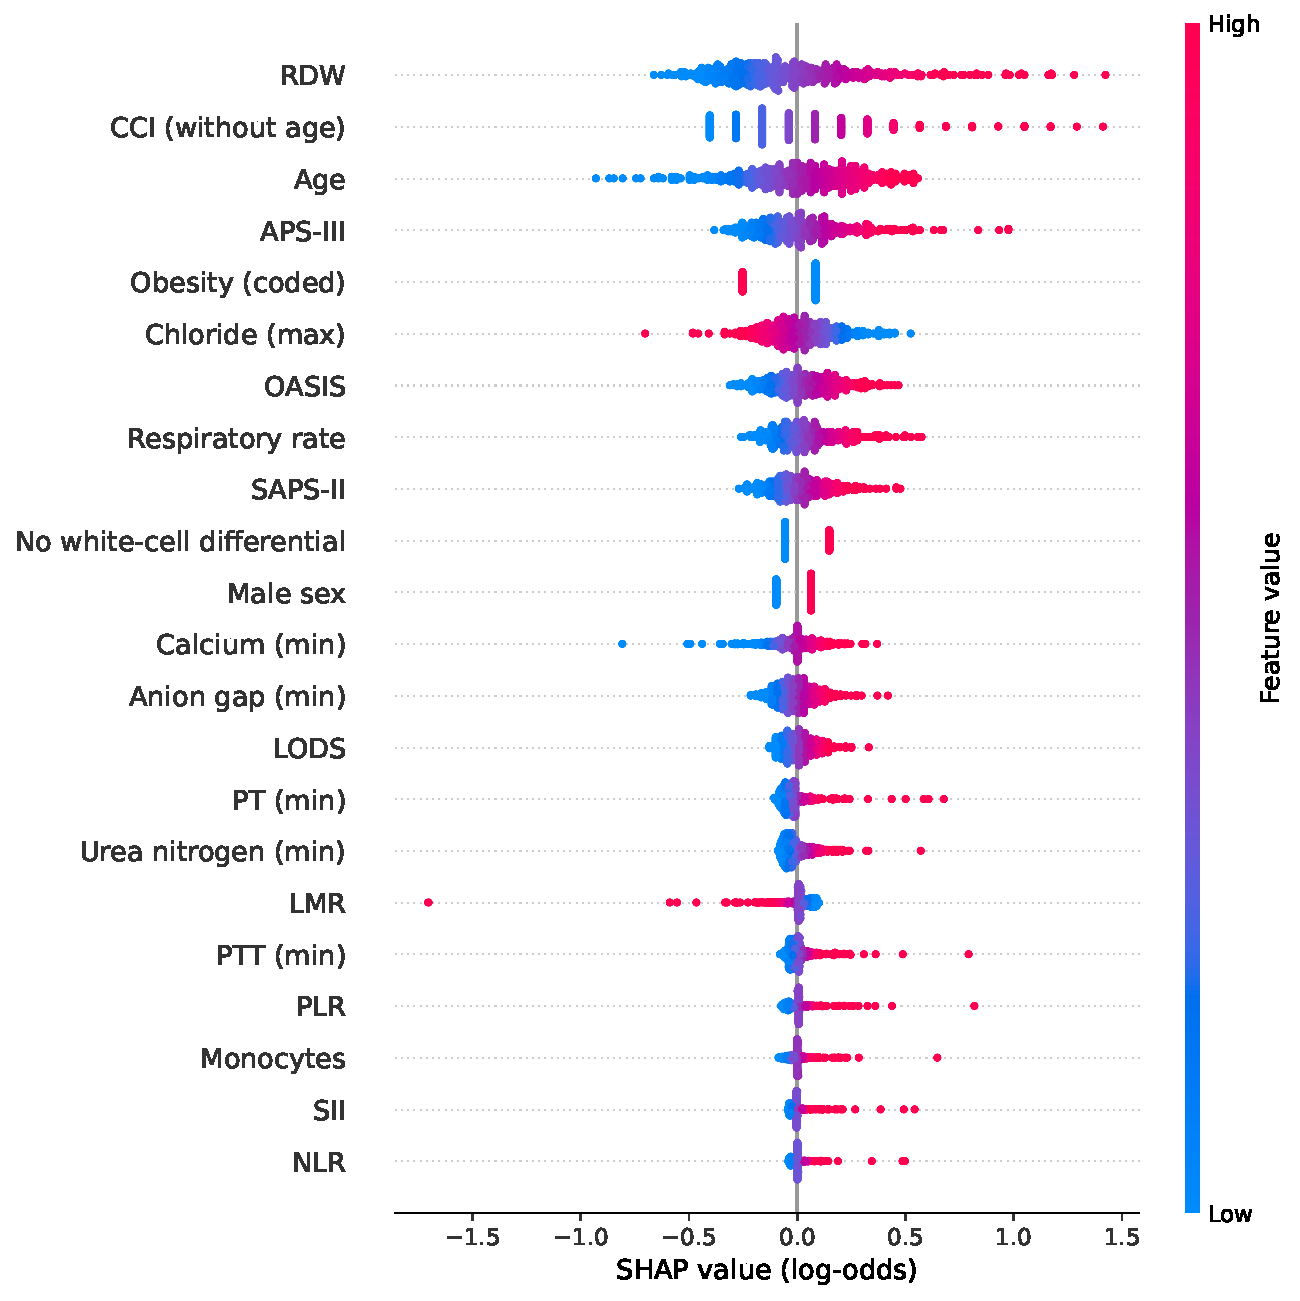
\includegraphics[width=0.8\textwidth]{figures/figC6_shap_beeswarm_clin_holdout.pdf}
\caption{SHAP summary of the frozen landmark LR (L2) on the held-out set (512 patients), log-odds scale, predictors ordered by mean $|\text{SHAP}|$. Colour shows the predictor value. For patients without a white-cell differential, the differential-derived variables take their imputed training means and appear as a cluster near zero. The corresponding plots for the reference cohort are in Supplementary S2.}
\label{fig:shap}
\end{figure}

\hypertarget{exploratory-extensions-1}{%
\subsection{Exploratory extensions}\label{exploratory-extensions-1}}

\emph{This section reports the extensions proposed in the project brief; all
results come from the development set.}

None of the extensions clearly improved on the static LR (Table 8). Stacking had
the highest AUROC, 0.805 against 0.799, a difference of 0.005 (95\% CI −0.001 to
0.011; p = 0.077, Holm-adjusted p = 1.00). Its direction was consistent, with
higher AUROC in 41 of 50 folds and a higher pooled out-of-fold AUROC in all five
repeats, and its out-of-fold calibration slope (1.05) was closer to 1 than that
of LR (0.90); its net benefit, however, was higher at only 31 of 56 thresholds.
Trajectory features entered every fit (median 4.5 selected per fold, range
1--13; SpO2 variability in 48 of 50 folds) but lowered AUROC slightly for LR, RF
and XGBoost (by 0.004, 0.001 and 0.002). Prior diagnoses were available for
1,183 development patients (57.8\%). Neither the burden variables nor the
embedding improved LR, and the embedding's small gain for RF (0.002 over the
static RF) came with a worse Brier score and a calibration slope further from 1
(1.35). Adding all extensions to the stacking ensemble changed AUROC by less
than 0.001. All comparisons had Holm-adjusted p = 1.00; the full results for 14
models are in Supplementary S12.

\begin{longtable}[]{@{}
  >{\raggedright\arraybackslash}p{(\columnwidth - 10\tabcolsep) * \real{0.2667}}
  >{\raggedright\arraybackslash}p{(\columnwidth - 10\tabcolsep) * \real{0.1500}}
  >{\raggedright\arraybackslash}p{(\columnwidth - 10\tabcolsep) * \real{0.0833}}
  >{\raggedright\arraybackslash}p{(\columnwidth - 10\tabcolsep) * \real{0.0833}}
  >{\raggedright\arraybackslash}p{(\columnwidth - 10\tabcolsep) * \real{0.1500}}
  >{\raggedright\arraybackslash}p{(\columnwidth - 10\tabcolsep) * \real{0.2667}}@{}}
\caption{Exploratory extensions on the landmark development set (fixed-parameter
recipe, 5 × 10 folds; ΔAUROC against the matched reference on the same folds,
with Nadeau--Bengio-corrected 95\% CI).}\tabularnewline
\toprule\noalign{}
\begin{minipage}[b]{\linewidth}\raggedright
Model
\end{minipage} & \begin{minipage}[b]{\linewidth}\raggedright
AUROC (mean ± SD)
\end{minipage} & \begin{minipage}[b]{\linewidth}\raggedright
AUPRC
\end{minipage} & \begin{minipage}[b]{\linewidth}\raggedright
Brier
\end{minipage} & \begin{minipage}[b]{\linewidth}\raggedright
Reference
\end{minipage} & \begin{minipage}[b]{\linewidth}\raggedright
ΔAUROC (95\% CI)
\end{minipage} \\
\midrule\noalign{}
\endfirsthead
\toprule\noalign{}
\begin{minipage}[b]{\linewidth}\raggedright
Model
\end{minipage} & \begin{minipage}[b]{\linewidth}\raggedright
AUROC (mean ± SD)
\end{minipage} & \begin{minipage}[b]{\linewidth}\raggedright
AUPRC
\end{minipage} & \begin{minipage}[b]{\linewidth}\raggedright
Brier
\end{minipage} & \begin{minipage}[b]{\linewidth}\raggedright
Reference
\end{minipage} & \begin{minipage}[b]{\linewidth}\raggedright
ΔAUROC (95\% CI)
\end{minipage} \\
\midrule\noalign{}
\endhead
\bottomrule\noalign{}
\endlastfoot
Static LR (L2) & 0.799 ± 0.026 & 0.607 & 0.151 & --- & --- \\
Static stacking & 0.805 ± 0.027 & 0.616 & 0.150 & Static LR & 0.005 (−0.001,
0.011) \\
LR + trajectories & 0.796 ± 0.026 & 0.602 & 0.153 & Static LR & −0.004 (−0.010,
0.003) \\
LR + diagnosis burden & 0.799 ± 0.027 & 0.607 & 0.151 & Static LR & 0.000
(−0.002, 0.002) \\
LR + burden + embedding & 0.796 ± 0.027 & 0.606 & 0.152 & LR + burden & −0.003
(−0.011, 0.004) \\
Stacking, all extensions & 0.805 ± 0.027 & 0.616 & 0.150 & Static stacking &
0.000 (−0.008, 0.008) \\
\end{longtable}

\hypertarget{discussion}{%
\section{Discussion}\label{discussion}}

\hypertarget{principal-findings}{%
\subsection{Principal findings}\label{principal-findings}}

Starting from the benchmark's framework, we corrected seven issues and evaluated
the result without leakage. The improved landmark model predicts one-year
mortality at a defined time, 24 h after ICU admission, from information
available then, and keeps the third of patients that the benchmark's blood-count
criterion excluded. Its discrimination was moderate, with a nested-CV AUROC of
0.801 and a confirmatory held-out AUROC of 0.750. Simple LR performed as well as
RF, XGBoost and SVM once every family was tuned inside the folds. The
benchmark's conclusion that RF is superior was not reproduced: its RF
configuration was significantly worse than the best model, and its training AUC
of 0.999 is reproduced by a forest of nine fully grown trees that memorises the
training data. The leading predictors were stable across cohorts and models:
RDW, comorbidity burden, age, illness severity and low chloride.

\hypertarget{impact-of-each-improvement}{%
\subsection{Impact of each improvement}\label{impact-of-each-improvement}}

Table 9 summarises what each modification changed. Some changed the conclusions;
others changed little and are reported for completeness.

\begin{longtable}[]{@{}
  >{\raggedright\arraybackslash}p{(\columnwidth - 2\tabcolsep) * \real{0.1333}}
  >{\raggedright\arraybackslash}p{(\columnwidth - 2\tabcolsep) * \real{0.8667}}@{}}
\caption{Observed effect of each improvement.}\tabularnewline
\toprule\noalign{}
\begin{minipage}[b]{\linewidth}\raggedright
Improvement
\end{minipage} & \begin{minipage}[b]{\linewidth}\raggedright
Observed effect
\end{minipage} \\
\midrule\noalign{}
\endfirsthead
\toprule\noalign{}
\begin{minipage}[b]{\linewidth}\raggedright
Improvement
\end{minipage} & \begin{minipage}[b]{\linewidth}\raggedright
Observed effect
\end{minipage} \\
\midrule\noalign{}
\endhead
\bottomrule\noalign{}
\endlastfoot
I1 Landmark at 24 h & Gives the model a defined time of use and removes a
criterion that depends on the future. The landmark model's nested-CV AUROC
(0.801) was similar to that of the reference cohort (0.786--0.791), although the
cohorts differ and this is not a controlled comparison. \\
I2 Keep patients without a differential & Retained 873 patients (34.1\%), whose
mortality was 28.6\% against 25.5\% (p = 0.09); the missingness indicator had OR
1.33 (1.04--1.71) but was selected in only 13 of 50 folds. Removing all
differential variables changed AUROC by +0.001 (−0.005, 0.007): no effect on
discrimination. \\
I3 Comorbidity timing & Changed the CCI for 843 reference patients; about half
of the myocardial-infarction diagnoses (304 of 611) rested only on acute codes.
AUROC did not change (+0.001). Relying on prior admissions only lowered AUROC by
0.014 and removed obesity from the model (50 to 4 of 50 folds), so the effect is
mainly on interpretation. \\
I4 Definitions & A fixed 365-day window gave 25.2\% mortality, against 42.8\%
when any recorded death is counted. The full hypertension definition removed a
spurious protective effect (OR 0.49 vs 1.07) without changing the LASSO
selection. With absolute counts, neutrophils were not selected at λ.1se. \\
I5 Nested evaluation & Selecting variables outside cross-validation overstated
AUROC by 0.008--0.030 in a single-repeat analysis (0.011 for the unpenalised
LR). Preprocessing leakage changed metrics by at most 0.001: no material effect
at this missingness. A single validation set could not separate the tuned
models, and the held-out estimate was 0.05 below the cross-validated one,
showing the variability of single-set estimates. \\
I6 Tuning all families & The largest effect. The benchmark's RF configurations
reached 0.724 and 0.767, significantly below the best model (0.791), whereas the
tuned RF (0.788) was equivalent to it. With tuning, the apparent advantage of RF
disappeared. \\
I7 Calibration and decision curves & Revealed differences that discrimination
hides: the R-default RF had slope 0.15, and the selected LR's slope moved from
1.11 out of fold to 0.82 on the held-out set, so recalibration is required. Net
benefit exceeded both default strategies at 53 of 56 thresholds. \\
\end{longtable}

\hypertarget{comparison-with-the-benchmark}{%
\subsection{Comparison with the benchmark}\label{comparison-with-the-benchmark}}

RF did not outperform the other families because, once all were tuned inside the
folds, the differences between them were within 0.005 in the reference cohort
and 0.008 in the landmark cohort. The benchmark's reported advantage of RF
rested on a single 263-patient validation set, on which a confidence interval
spans about ±0.05 (0.723--0.837 for its RF), and on a training AUC that reflects
memorisation rather than performance.

The landmark model's held-out AUROC of 0.750 is below the benchmark's 0.780, but
the two numbers are not comparable, for four reasons. First, the cohorts differ:
the landmark cohort includes patients without a white-cell differential, does
not exclude patients with short hospital stays, and comes from a later data
release. Second, the outcomes probably differ: the benchmark's abstract names
in-hospital death, yet its mortality of 38.2\% is far above in-hospital
mortality in our cohort and is consistent with counting deaths without a fixed
window. Third, our estimate is confirmatory: the model was frozen before a
single held-out evaluation, whereas the benchmark's validation set also served
for model selection. Fourth, the held-out confidence interval (0.702--0.797)
includes 0.780, and the same pipeline gave 0.786--0.791 in the reference cohort
and 0.801 under nested cross-validation in the landmark cohort. The appropriate
conclusion is that discrimination is moderate, about 0.75--0.80, in both
studies.

\hypertarget{biological-plausibility-of-the-main-predictors}{%
\subsection{Biological plausibility of the main
predictors}\label{biological-plausibility-of-the-main-predictors}}

\textbf{RDW} was the strongest predictor in every analysis, in agreement with
the benchmark and with studies linking RDW to mortality in critically ill
patients \parencite{bazick2011}. Elevated RDW reflects heterogeneous
erythropoiesis driven by inflammation, oxidative stress, nutritional deficiency
and renal dysfunction, which are prevalent in long-standing diabetes.
\textbf{CCI} captures the cardiovascular and renal burden that typically
accompanies DN \parencite{feldman2019}, and its importance persisted after
recomputing it from chronic codes only. \textbf{Low chloride}, associated with
higher risk in both our work and the benchmark, is a recognised marker of poor
outcome in critical illness \parencite{tani2012}. The apparently protective
effect of \textbf{coded obesity} was concentrated in patients whose obesity code
appeared only during the index admission: their one-year mortality was 18.8\% (n
= 416), against 26.4\% (n = 443) when obesity was coded in a prior admission and
28.6\% (n = 1,698) without an obesity code. This suggests a documentation
artefact rather than a true ``obesity paradox'', and it should be tested with
measured body-mass index.

\hypertarget{limitations}{%
\subsection{Limitations}\label{limitations}}

\begin{itemize}
\tightlist
\item
  \textbf{Single-centre, retrospective data and no external validation.} The
  landmark held-out set has only 136 events, which limits the precision of the
  confirmatory estimate.
\item
  \textbf{DN identified from ICD codes.} Their accuracy is unknown, and codes
  carry no timestamps. The main landmark estimate assumes that chronic
  index-admission codes were present at admission; using prior admissions only
  lowers AUROC to about 0.787.
\item
  \textbf{Unstable calibration.} The slope was 1.11 out of fold and 0.82 on the
  held-out set, so the model must be recalibrated before use in a new
  population.
\item
  \textbf{Only first-day features.} Treatments were not used, within-day
  dynamics were tested only in the exploratory extensions, and cause of death is
  unavailable.
\item
  \textbf{Exploratory extensions.} They were run after the held-out results had
  been seen, with fixed rather than tuned hyperparameters, and were not
  evaluated on held-out data; a small gain from stacking cannot be excluded.
\item
  \textbf{Non-blind model selection in the reference cohort.} The selection rule
  was written after exploratory analyses of the reference cohort, and its
  held-out set had been used in those analyses; only the landmark analyses were
  fully pre-specified.
\end{itemize}

\hypertarget{future-work}{%
\subsection{Future work}\label{future-work}}

\begin{itemize}
\tightlist
\item
  \textbf{Temporal validation.} Train on earlier and test on later MIMIC-IV year
  groups, and validate externally in data with one-year follow-up.
\item
  \textbf{Recalibration and thresholds.} Recalibrate the model in the target
  population and choose thresholds for specific clinical uses.
\item
  \textbf{Objective measurements.} Use measured body-mass index to test the
  obesity finding.
\item
  \textbf{Richer predictors and models.} Add HbA1c and treatment variables, and
  test stacking with tuned base learners on new data. Clinical notes, SHAP
  interaction values and counterfactual explanations, also proposed for this
  project, were not run.
\end{itemize}

\hypertarget{conclusion}{%
\section{Conclusion}\label{conclusion}}

We took a published machine-learning framework for one-year mortality in ICU
patients with diabetic neuropathy and corrected its cohort definition, predictor
definitions and evaluation. The resulting landmark model uses only information
available 24 h after ICU admission and was frozen before a single confirmatory
evaluation. Under leakage-free nested cross-validation, LR matched tree
ensembles, and the benchmark's reported RF advantage reflected an overfitted
configuration and a single small validation set. RDW, comorbidity burden and age
were consistently the strongest predictors. Exploratory trajectory features,
diagnosis embeddings and stacking added little or nothing to discrimination. The
landmark model's discrimination is moderate (AUROC 0.75--0.80), and it should be
recalibrated locally before clinical use.


\printbibliography

\clearpage
\hypertarget{supplementary-material}{%
\section{Supplementary material}\label{supplementary-material}}

\begin{itemize}
\tightlist
\item
  \textbf{S1. Four cohort definitions.} Four readings of ``first ICU
  admission at first hospitalization'', with counts and one-year
  mortality.
\item
  \textbf{S2. Reference cohort: complete results.} Nested
  cross-validation of all nine configurations, LASSO selection
  frequencies, the model-selection steps, the secondary held-out
  estimate, thresholds, decision curves, coefficients and SHAP.
\item
  \textbf{S3. Full baseline tables} of the reference and landmark
  cohorts.
\item
  \textbf{S4. Comparison with the benchmark's Table 1} and the
  mixed-unit diagnostic for the white-cell differential.
\item
  \textbf{S5. Hypertension definitions} and their associations with
  one-year death.
\item
  \textbf{S6. LASSO cross-validation curve and coefficient path.}
\item
  \textbf{S7. Exploratory single-split results} (all models, paired
  DeLong comparisons, thresholds, calibration, LASSO-only nesting).
\item
  \textbf{S8. Comorbidity-timing recode}: acute codes removed and
  changes in each comorbidity.
\item
  \textbf{S9. Implementation details.} Global random seed 42 and repeat
  seeds; LASSO implementation (λ grid of 100 values from
  \(\lambda_{\max} = \max_j \lvert\mathbf{x}_j^\top(\mathbf{y} - \bar y)\rvert / n\)
  down to \(10^{-4}\lambda_{\max}\); liblinear intercept feature set to
  1,000 so that the intercept penalty is negligible; binomial deviance
  as the criterion, whereas the benchmark's text names mean squared
  error but its figure shows binomial deviance); the benchmark's
  hyperparameters and their mapping to scikit-learn and xgboost; all
  tuning grids.
\item
  \textbf{S10. Benchmark-style versus leakage-free preprocessing}: LASSO
  selection, validation AUROC and SHAP.
\item
  \textbf{S11. Code availability and reproducibility}: pipeline scripts,
  seeds and the frozen-model specification.
\item
  \textbf{S12. Exploratory extensions: complete results.} All 14 models
  (LR, RF, XGBoost and stacking with static, trajectory, burden and
  embedding inputs), all 45 paired comparisons, pooled out-of-fold
  calibration, decision-curve comparisons and trajectory-feature
  selection frequencies.
\end{itemize}


\end{document}
